% ============================================================
% The Dynamical Substrate Law:
%   Substrate-Locality of DI-Bit Currents at Vertex-Aligned
%   Reading C in the 600-Cell
% Conscious Point Physics Flagship Paper Series (F-line)
%
% Version 1.0 -- 24 May 2026 (Session 142, Patch 0570 — v1.0 SHIP)
%   v1.0 SHIP: structurally-grounded sketch-document Layer 3 flagship
%   framework preprint with publication-grade hardened components but
%   non-publication-grade umbrella theorem. Paper compiles to 33 pages.
%   Author email: drthomas@protonmail.com (updated at Patch 0569a).
%
%   Build history:
%     Patch 0554 — paper skeleton created (preamble + section headers
%       + title + abstract draft + 5 Open Problem placeholders)
%     Patches 0556-0565 — 10-Patch body-content assembly arc:
%       Patch 0556 §1 introduction; Patch 0557 §2 F.1 sub-question;
%       Patch 0558 §3 framework primitives; Patch 0559 §4 Mechanism A;
%       Patch 0560 §5 first-shell identities (FIRST integration Patch,
%         importing Patches 0551+0552 hardened theorems);
%       Patch 0561 §6 perturbation-locality (SECOND integration Patch,
%         importing Patch 0550 hardened theorem);
%       Patch 0562 §7 substrate-locality umbrella theorem
%         (constructed from §5+§6 inputs at sketch-document Layer 3);
%       Patch 0563 §8 Layer 3 stack (collation with explicit Layer
%         hierarchy table);
%       Patch 0564 §9 open questions body (5 Open Problem statements);
%       Patch 0565 §10 conclusion (final body-section Patch);
%     Patch 0566 — bibliography body (13 \bibitem entries; Option B:
%       explicit entries with body unchanged)
%     Patch 0567 — pre-v1.0 final polish: date metadata + CHANGELOG
%       comment + abstract Open Problem count corrected from 3 to 5
%     Patches 0568-0569e — v0.9 → v1.0 SHIP-cycle reviewer engagement:
%       Patch 0568 Round 1 archival + synthesis (Copilot + ChatGPT
%         + Grok letters; 1 MUST-ADDRESS + 4 SHOULD-ADDRESS + 5
%         CAN-DEFER + 2 DECLINED items classified)
%       Patch 0569 Round 1 multi-edit response (8 atomic LaTeX edits
%         implementing 5 reviewer-cycle items: thermodynamic-arrow
%         framing triple-coverage at abstract + §1.1 + §10 +
%         executive summary; §7.3 Step 3 representation-theoretic
%         justification)
%       Patch 0569a Round 2 reviewer-driven adjustments + author
%         email update (4 atomic edits)
%       Patch 0569b Round 3 reviewer-driven adjustments (5 atomic
%         edits inc. Figure 8.1 TikZ dependency-graph in §8.2 +
%         bold declarative in §1 executive summary)
%       Patches 0569c-0569e Rounds 4-6 archival + diagnostic-framing
%         + recurring-pattern documentation + diagnostic resolution
%         (TikZ-rendering processing artifact identified at R4,
%         confirmed at R6 via PDF upload protocol change; no `.tex`
%         edits at these Patches)
%     Patch 0570 — v1.0 SHIP: \date{} update + CHANGELOG update +
%       compiled PDF committed as frozen reference for v1.0 milestone
%
%   The three publication-grade hardened theorem artifacts at
%   `series_umbrella/series_substrate_chirality_arc/dynamical_substrate_law/hardened_theorems/`
%   (Patches 0550 + 0551 + 0552, 741 lines LaTeX combined) supplied
%   §5 and §6 body content as direct integration inputs.
%
%   v1.0 SHIP cross-reviewer position (multi-round convergent verdict):
%     Grok Round 1: EXPLICIT v1.0 SHIP-acceptable
%     Copilot Round 1: implicit SHIP-acceptable with tier-ranked
%       recommendations
%     ChatGPT Round 1 → 2 → 3 → 4 → 5 → 6: monotonic verdict
%       improvement from "NOT yet publication-grade flagship overall"
%       to "substantially more credible, rigorous, and publishable
%       than all earlier versions" (R6 strongest-positive)
%
%   Post-v1.0 trajectory (v2.0+ candidate follow-up Patches):
%     OPEN-FP-F1-3 — G1 publication-grade hardening (ChatGPT R1-R6
%       convergent "single highest-value next action")
%     OPEN-FP-F1-2 — Layer 4 axiomatic derivation of Mechanism A
%     OPEN-FP-F1-6 — Prose-density tightening (registered at
%       Patch 0569e from ChatGPT R6)
%     F.1-condensed companion paper — Theorem 6.1 + Corollary 6.2 +
%       Theorem 7.1 focused with minimal CPP interpretation
%       (registered at Patch 0569e from ChatGPT R6)
%
%   Anti-priorities sustained throughout assembly + reviewer cycle:
%     preserve Layer distinction + conditionality + open higher-order
%     questions; do not erase uncertainty structure during paper
%     polishing. Discipline named explicitly at §8.3 closing paragraph
%     as "anti-erasure discipline"; operationalised at three concrete
%     points in §10. 5-Open-Problem commitment preserved end-to-end.
%     Calibration discipline at Patches 0569 → 0569e: no theorem
%     statements modified, no proofs modified (Patch 0569a Edit C
%     added clarification AFTER existing Lemma 6.3.1 proof), no Open
%     Problems modified, no hardened_theorems/*.tex source artifacts
%     modified, no bibliography body modified.
% ============================================================

\documentclass[11pt,letterpaper]{article}
\usepackage[utf8]{inputenc}
\usepackage[margin=1in]{geometry}
\usepackage[T1]{fontenc}
\usepackage{amsmath,amssymb,amsfonts,amsthm}
\usepackage{graphicx}
\usepackage{tikz}
\usetikzlibrary{positioning,calc,arrows.meta,shapes.geometric}
\usepackage{xcolor}
\usepackage{hyperref}
\usepackage{booktabs}
\usepackage{array}
\usepackage{enumitem}
\usepackage{float}
\usepackage[font=small, labelfont=bf]{caption}
\usepackage{parskip}
\usepackage{mdframed}

\hypersetup{
    colorlinks=true,
    linkcolor=blue,
    citecolor=blue,
    urlcolor=blue
}

\newtheorem{theorem}{Theorem}[section]
\newtheorem{proposition}[theorem]{Proposition}
\newtheorem{lemma}[theorem]{Lemma}
\newtheorem{corollary}[theorem]{Corollary}
\newtheorem{conjecture}[theorem]{Conjecture}
\newtheorem{definition}[theorem]{Definition}
\newtheorem{remark}[theorem]{Remark}
\newtheorem{claim}[theorem]{Claim}
\newtheorem{openproblem}{Open Problem}

% Notation conventions inherited from Capotauro v2.0 + SF-4 +
% the F.1 hardened theorem artifacts (Patches 0550 + 0551 + 0552)
\newcommand{\phig}{\varphi}
\newcommand{\nhat}{\hat{n}}
\newcommand{\vhost}{v_{\text{host}}}
\newcommand{\jDInet}{\vec{j}_{DI}^{\,\text{net}}}
\newcommand{\omegaPCD}{\vec{\omega}_{PCD}}
\newcommand{\sigcycle}{\sigma_{\text{cycle}}}
\newcommand{\Mthermo}{|M^{\text{thermo}}|}
\newcommand{\DeltapLR}{\Delta p_{LR}}
\newcommand{\Ih}{I_h}
\newcommand{\PTI}{P_{TI}}
\newcommand{\Zbw}{\mathrm{ZBW}}
\newcommand{\bigO}[1]{\mathcal{O}(#1)}
\newcommand{\Findd}{\mathrm{DSL}}

\title{The Dynamical Substrate Law:\\
Substrate-Locality of DI-Bit Currents at\\
Vertex-Aligned Reading~C in the 600-Cell}

\author{Dr.~Thomas Lee Abshier, ND\\
\small Hyperphysics Institute\\
\small \texttt{drthomas@protonmail.com}\\
\\
\small with AI co-authorship:\\
\small Claude Opus (Anthropic) --- primary mathematical co-author\\
\small ChatGPT (OpenAI), Copilot (Microsoft), Grok (xAI) --- review and calibration
}

\date{Version 1.0 --- 24 May 2026\\[3pt]{\small\itshape Structurally-grounded sketch-document Layer 3 flagship framework preprint with publication-grade hardened components but non-publication-grade umbrella theorem.}}

\begin{document}

\maketitle

% ============================================================
% Abstract --- draft v0.1, refined at later assembly Patches
% ============================================================
\begin{abstract}
We establish the substrate-locality property for DI-bit currents on the 600-cell substrate at vertex-aligned Reading~C: under Mechanism~A (the propagation-rate-asymmetry primitive $r(\hat{e}) = r_0(1 + \delta\,\hat{e}\cdot\nhat)$) and the framework-local current construction at first order in $\delta$, the substrate net DI-bit current at any host vertex $\vhost$ depends only on first-shell content. The result is proved at sketch-document Layer~3 in three steps: (i)~the host-to-first-shell unit-direction projection $\hat{u}_i \cdot \nhat = -1/(2\phig)$ is uniform across all twelve first-shell neighbours (Theorem~\ref{thm:host-first-shell-projection}); (ii)~the first-shell-to-first-shell edge-direction projection $\hat{e}_{ij} \cdot \nhat = 0$ vanishes for any pair of first-shell vertices (Theorem~\ref{thm:first-shell-perpendicularity}); (iii)~the perturbation-theory propagation rule confines the $\bigO{\delta^n}$ coefficient of the substrate current to graph-distance-$n$ edges in the 600-cell edge graph (Theorem~\ref{thm:perturbation-locality}, with shell-locality Corollary~\ref{cor:shell-locality}).
The three load-bearing identities --- host-to-first-shell uniform projection, first-shell-to-first-shell perpendicularity, and the perturbation-theory propagation rule (with shell-locality corollary) --- are hardened at publication-grade rigor with explicit hypothesis tracking and five-class exclusion enumeration each.
We make the scope qualifier --- perturbative locality under Mechanism~A and the framework-local current construction at $\bigO{\delta^1}$ --- structurally inseparable from the theorem statements.
Five open higher-order questions are registered (Section~\ref{sec:open-questions}); the three core extension/derivation questions are: extension to $\bigO{\delta^2}$ (Open~Problem~\ref{op:delta-squared}); Layer~4 axiomatic derivation of Mechanism~A from the eleven CPP primitive axioms~A1--A11 (Open~Problem~\ref{op:layer4-mechanism-a}); and publication-grade hardening of the first-shell inner-product primitive G1 (Open~Problem~\ref{op:g1-hardening}). Two additional research-direction-choosing questions register the broader chirality continuum (Open~Problem~\ref{op:sector5-schema}, Sector-5 schema instantiation) and Reading~C-variant programmes (Open~Problem~\ref{op:non-vertex-aligned-c}, non-vertex-aligned Reading~C variants).
\textbf{Scope of the closure}: the present paper establishes \emph{substrate-locality structure} (the closed-form first-order DI-bit current at the host vertex) supporting the candidate thermodynamic-arrow mechanism for manifestation~(iv) of OPEN-SD-CHIR-PRIMITIVE. The full thermodynamic-arrow emergence in the conventional physics sense --- entropy production, irreversible coarse-graining, statistical-mechanics emergence --- is the candidate mechanism narrative supported by, but not derived from, the present paper's result; the emergence layer is registered as future work beyond the present paper's framework qualifiers.
The paper integrates the F.1 sub-question of the OPEN-SD-CHIR-PRIMITIVE manifestation~(iv) trajectory and is the temporal-sector analog to the Capotauro~v2.0 spatial-sector substrate-locality theorem, with which it shares the structural constant $-1/(2\phig)$.
\end{abstract}

\tableofcontents

% ============================================================
% §1 Introduction and motivation
%   Body to be added at Patch 0555.
%   Primary source: F1_subquestion_pcd_orientation_link.md §1
%   (with framing for outer audience).
%   Approximate target: 3-4 pages.
% ============================================================
\section{Introduction and motivation}
\label{sec:introduction}

% [Body added at Patch 0556. Outer comment header above anticipated
%  Patch 0555 for this body; the audit took that slot, so body landed
%  at Patch 0556 per the Patch 0554-vs-0555 sequencing record (§16.5
%  of F1_phase2_foundations_work.md).]

\paragraph{Executive summary.}
This paper establishes the substrate-locality property of DI-bit currents at vertex-aligned Reading~C in the 600-cell substrate. The principal result is Theorem~\ref{thm:substrate-locality}: the net DI-bit current at any host vertex $\vhost$ at first order in the propagation-rate-asymmetry parameter $\delta$ is given in closed form by $\jDInet(\vhost) = (6\delta/\phig^2)\hat{n} + \bigO{\delta^2}$, depending only on first-shell content. The result is proved at sketch-document Layer~3 (\S\ref{sec:substrate-locality-theorem}) by assembling three publication-grade building-block theorems hardened in separate `.tex' artifacts (\S\S\ref{sec:first-shell-identities}--\ref{sec:perturbation-locality}): the host-to-first-shell uniform projection (Theorem~\ref{thm:host-first-shell-projection}), the first-shell-to-first-shell perpendicularity (Theorem~\ref{thm:first-shell-perpendicularity}), and the perturbation-locality propagation rule (Theorem~\ref{thm:perturbation-locality}, with shell-locality Corollary~\ref{cor:shell-locality}). The substrate-locality structure supports a candidate thermodynamic-arrow mechanism (manifestation~(iv) of the chirality continuum's substrate-direction primitive); the full emergence layer is registered as future work. \textbf{The present paper does not derive entropy production, coarse-graining, or macroscopic irreversibility}; those derivations are future work beyond the present paper's framework qualifiers. Five open higher-order questions are registered (\S\ref{sec:open-questions}).

\subsection{Position in the CPP corpus and the chirality continuum}
\label{sec:position-in-cpp}

The Conscious Point Physics (CPP) programme aims to derive Standard Model physics from the discrete geometry of the 600-cell polytope, with zero free parameters. The framework posits a substrate of Conscious Points (CPs) executing Polarize $\to$ Capture $\to$ Depolarize (PCD) cycles, with Dipole Points (DPs) as composite intermediate objects, governed by eleven primitive axioms A1--A11 (\textit{Tetrahedrons All the Way Down}, Abshier 2026; central bibliography at \texttt{bibliography/cpp\_references.bib}, to be cited via \texttt{\textbackslash cite} at Patch 0566+).

A central long-term programme target of CPP is the \emph{chirality continuum}: relating handedness in the spatial sector (parity violation, neutrino chirality structure, weak isospin assignment) to handedness in the temporal sector (irreversibility, thermodynamic causal arrow, cosmological-vacuum asymmetry). The chirality continuum architecture, established in the Capotauro v2.0 paper (\texttt{chirality\_continuum.tex}), identifies five manifestations of an open substrate-direction primitive (\texttt{OPEN-SD-CHIR-PRIMITIVE}):
\begin{itemize}[leftmargin=2em]
\item[(i)] parity violation (closed at Capotauro v2.0);
\item[(ii)] neutrino chirality structure (closed at Capotauro v2.0 + SF-4 v1.0);
\item[(iii)] weak isospin assignment (closed at Capotauro v2.0);
\item[(iv)] thermodynamic causal arrow --- \emph{the present paper's target at the substrate-locality level};
\item[(v)] cosmological-vacuum asymmetry (future work; F.3 trajectory).
\end{itemize}

The Capotauro v2.0 paper closed the substrate-locality theorem for manifestations (i)--(iii) (spatial-sector). The present paper extends the substrate-locality property to manifestation (iv) (temporal-sector) via the \emph{dynamical substrate law}: the substrate net DI-bit current at any host vertex of the 600-cell depends only on first-shell content at vertex-aligned Reading~C, under Mechanism~A (defined below) and the framework-local current construction at first order in the perturbation parameter $\delta$.

What this paper establishes at manifestation~(iv) is the \emph{substrate-locality structure} --- the closed-form expression for the net DI-bit current at the host vertex, depending only on first-shell content at first order in $\delta$. This substrate-locality structure \emph{supports} the candidate thermodynamic-arrow mechanism (asymmetric DI-bit arrival at the host vertex $\to$ capture-phase bias in the PCD cycle $\to$ preferred PCD orientation $\to$ macroscopic arrow asymmetry). The full mechanism narrative --- from substrate-locality structure to thermodynamic-arrow emergence in the conventional physics sense (entropy production, irreversible coarse-graining, statistical-mechanics emergence) --- requires additional derivation steps that are not the present paper's scope and are registered as future work. The present paper's closure is at the \emph{substrate-locality level}; the thermodynamic-arrow emergence layer is conjectured (via the mechanism narrative) but not derived.

Both papers share the structural constant $-1/(2\phig)$, where $\phig = (1 + \sqrt{5})/2$ is the golden ratio. At vertex-aligned Reading~C in the 600-cell, the inner product between a host vertex's unit vector and any first-shell neighbour's unit vector equals $-1/(2\phig)$ uniformly across all twelve first-shell directions (Theorem~\ref{thm:host-first-shell-projection} of the present paper, hardened at publication-grade Layer~3 per the Patch 0552 hardened theorem artifact). The same constant governs the Capotauro v2.0 spatial-sector substrate-locality theorem (Capotauro v2.0 \S3). The structural parallel is not coincidental: it reflects the same first-shell first-order geometric constraint operating in both the spatial and temporal sectors of the chirality continuum.

\subsection{The F.1 sub-question as a programme gate}
\label{sec:f1-as-programme-gate}

The \texttt{OPEN-SD-CHIR-PRIMITIVE} substrate-direction primitive carries a specific load-bearing question for the temporal-sector manifestation (iv): does the link $\hat{n} \mapsto \omegaPCD$ have substrate-mechanism support, or is the PCD-cycle-orientation pseudovector $\omegaPCD$ an independent primitive parallel to $\hat{n}$? Three closure scenarios were identified at scoping:
\begin{itemize}[leftmargin=2em]
\item \textbf{Scenario A (positive)}: the link $\hat{n} \mapsto \omegaPCD$ is derived via substrate-mechanism. The PCD-cycle-orientation pseudovector at the host vertex satisfies $\omegaPCD(\vhost) = \sigma \cdot \hat{n}$ with $\sigma \in \{+1, -1\}$ a global sign convention, with the alignment derived rather than posited.
\item \textbf{Scenario B (negative)}: the PCD-cycle-orientation is an independent primitive, not derivable from substrate-mechanism. The chirality continuum umbrella refines to a three-way structure (spatial-direction primitive, temporal-direction primitive, and their alignment as a separate convention).
\item \textbf{Scenario C (partial)}: partial derivation closure; requires additional framework input beyond the existing CPP axiom set.
\end{itemize}

The F.1 sub-question is the load-bearing prerequisite gate for the F.2 + F.3 trajectories (manifestations (iv) substantive content and (v) cosmological-vacuum asymmetry). Only with Scenario~A closure can the chirality continuum architecture proceed via the qDP/eDP precedent template established at Capotauro v2.0 \S20. Scenario~B closure would require alternative architecture; Scenario~C closure would require an additional framework input.

This paper establishes the substrate-locality component required for Scenario~A closure under a specific framework: the Reading~C + 600-cell + Mechanism~A minimal-local-first-order framework, at \emph{sketch-document Layer~3} rigor. The substrate-locality component is the substrate-mechanism support for the $\hat{n} \mapsto \omegaPCD$ link via the closed-form first-order DI-bit current (Theorem~\ref{thm:substrate-locality}); the coupling from substrate current to macroscopic PCD orientation at the host vertex --- i.e., the full $\hat{n} \mapsto \omegaPCD$ derivation including the mechanism narrative for thermodynamic-arrow emergence --- is supported by, but not derived from, the present paper's result, and is registered as future work. The Layer-distinction discipline is operationally important and is sustained throughout the paper (see \S\ref{sec:layer3-stack}). Layer~4 axiomatic derivation of Mechanism~A from the eleven CPP primitive axioms A1--A11 remains open as a long-term programme target (Open Problem~\ref{op:layer4-mechanism-a}).

\subsubsection*{Mechanism A in brief}

Mechanism~A is the propagation-rate asymmetry primitive: the DI-bit (Dimensional Increment bit, the discrete unit of information propagation between CPs per CPP axiom A1) acquires a small direction-correlated propagation-rate asymmetry under the substrate primitive $\hat{n}$. Formally,
\begin{equation}
r(\hat{e}) = r_0 \left(1 + \delta \cdot \hat{e} \cdot \hat{n}\right),
\label{eq:mechanism-a}
\end{equation}
where $r(\hat{e})$ is the DI-bit propagation rate along unit-direction $\hat{e}$, $r_0$ is the $H_4$-idealized substrate rate, $\delta$ is the perturbation parameter (small, $|\delta| \ll 1$), and $\hat{n}$ is the substrate primitive 4D direction. DI-bits propagating in the $+\hat{n}$ direction propagate at rate $r_0(1 + \delta)$; in the $-\hat{n}$ direction at $r_0(1 - \delta)$; in any tangent direction ($\hat{e} \cdot \hat{n} = 0$) at the idealized rate $r_0$. The PCD cycle's Polarize $\to$ Capture $\to$ Depolarize sequence at each CP couples to this asymmetric flow, inducing a definite cycle-orientation $\omegaPCD$ aligned with $\hat{n}$. Mechanism~A is the leading candidate by structural analogy to Reading~C edge-length perturbation (Capotauro v2.0 \S2.3): both involve a direction-correlated propagation-asymmetry of substrate quantities controlled by a single small parameter ($\varepsilon$ in Capotauro, $\delta$ in the present paper).

\subsection{Sketch Layer 2 to Layer 3 trajectory recap}
\label{sec:trajectory-recap}

The substrate-locality theorem at Reading~C was developed across a multi-phase sketch trajectory spanning Sessions 137--142 (calendar months April--May 2026). The trajectory's high-level structure was:

\begin{itemize}[leftmargin=2em]
\item \textbf{Phase 1: initial substrate-mechanism scoping} (Patches 0510--0522, approximately). Three candidate mechanisms identified: Mechanism~A (propagation-rate asymmetry), Mechanism~B (substrate-orientation field with gauge-like PCD coupling), and Mechanism~C (position-dependent clock-skew). Mechanism~A established as the leading candidate by structural analogy to Reading~C edge-length perturbation.
\item \textbf{Phase 2: foundations work} (Patches 0523--0537). Consolidation of Mechanism~A as the leading candidate, with sketch-document Layer~2 derivation of seven foundational sub-results (first-shell net DI-bit current vanishing at $H_3 = I_h$ symmetric configurations; isolated-host vs.\ embedded-host scoping; matter-state independence; substrate-locality temporal extension; and others) culminating in a sketch-level closure conclusion for Mechanism~A under the minimal-local-first-order realization framework.
\item \textbf{First reviewer-pause cycle (sketch Layer~2 closure)}: Patches 0538 (reviewer-pause checkpoint document submission) $\to$ 0539a (calibration response Patch processing verbatim reviewer feedback from ChatGPT, Copilot, Grok) $\to$ 0539 (F.1 sub-question status upgrade to ``substantive sketch-level closure at Layer~2 under the minimal-local-first-order realization framework''). The first reviewer-pause cycle established the cycle-discipline workflow per \texttt{templates/reviewer\_pause\_template.md}.
\item \textbf{Layer~3 promotion arc} (Patches 0540--0546 + 0548a). Seven structural targets identified at the Patch 0540 scoping document and closed across Patches 0541--0546 at sketch-document Layer~3, with the seventh target retroactively recognized at Patch 0546 and consolidated as a standalone artifact at Patch 0548a per the \S5.3 anti-bundling discipline. Three load-bearing identities/theorems emerged: Identity~I1 (host-to-first-shell uniform projection $-1/(2\phig)$), Identity~G3 (first-shell-to-first-shell perpendicularity $\hat{e}_{ij} \cdot \hat{n} = 0$), and Theorem 3.3.3 (perturbative-locality propagation rule at order $\bigO{\delta^n}$ confined to graph-distance-$n$ edges, with shell-locality Corollary 3.3.4 specialising to $\bigO{\delta^1}$).
\item \textbf{Second reviewer-pause cycle (Layer~3 closure)}: Patches 0547--0549. The second reviewer-pause cycle (parallel structure to the first) upgraded the F.1 sub-question status to \emph{``structurally-grounded sketch-document Layer~3 closure under the Reading~C + 600-cell + Mechanism~A minimal-local-first-order framework, pending Layer~4 axiomatic derivation, $\bigO{\delta^2}$ extension, and publication-grade hardening''} per cross-reviewer-convergent feedback weighting (ChatGPT precision on framework scope + Copilot inclusivity on pending items).
\item \textbf{Publication-grade hardening trio} (Patches 0550--0552). Three publication-grade Layer~3 hardenings landed in dedicated \texttt{.tex} artifacts at \texttt{flagship\_papers/dynamical\_substrate\_law/\linebreak hardened\_theorems/}: perturbation-locality propagation rule (Patch 0550, Theorem 3.3.3 + Corollary 3.3.4), first-shell-to-first-shell perpendicularity (Patch 0551, Theorem 4.1.1 / Identity G3), and host-to-first-shell uniform projection (Patch 0552, Theorem 4.2.1 / Identity I1). Each carries explicit hypothesis tracking and a five-class exclusion enumeration; the trio's combined output is 741 lines of LaTeX across 21 PDF pages.
\end{itemize}

\textbf{Status as of the present paper}: \emph{structurally-grounded sketch-document Layer~3 closure under the Reading~C + 600-cell + Mechanism~A minimal-local-first-order framework, pending Layer~4 axiomatic derivation, $\bigO{\delta^2}$ extension (cross-reference: \texttt{OPEN-SS-B1q6} in the open-problems registry), and publication-grade hardening of identity G1} (the 600-cell first-shell uniform inner-product primitive, which is a shared dependency of Theorems~\ref{thm:host-first-shell-projection} and~\ref{thm:first-shell-perpendicularity}; tracked as Open Problem~\ref{op:g1-hardening}).

The trajectory recap above is high-level; per-Patch documentation lives in the \texttt{documentation\_suite/} files (Tier~4 reasoning, Tier~3 vignettes, Tier~2 transactions) and in the \texttt{sketches/F1\_phase2\_foundations\_work.md} \S16 cross-reference chronology (consolidated at Patch 0555).

\subsection{Paper roadmap and Layer-distinction discipline}
\label{sec:roadmap-and-layer-discipline}

\subsubsection*{Section-by-section roadmap}

\begin{itemize}[leftmargin=2em]
\item[\S\ref{sec:subquestion}] formalizes the F.1 sub-question: precise statement of the link $\hat{n} \mapsto \omegaPCD$ derivation question, the three closure scenarios, and the minimal-local-first-order realization framework that makes Scenario~A derivable.
\item[\S\ref{sec:framework-primitives}] defines the framework primitives: CPP primitive axioms A1--A11 (recap); the 600-cell substrate at vertex-aligned Reading~C; first-shell geometric primitives G1 (uniform inner product) and G2 (icosahedral first-shell structure); the DI-bit and Mechanism~A coupling.
\item[\S\ref{sec:mechanism-a}] codifies Mechanism~A as framework axiom and the framework-local current construction at first order in $\delta$. (Layer~4 axiomatic derivation of Mechanism~A from CPP A1--A11 is deferred to Open Problem~\ref{op:layer4-mechanism-a}.)
\item[\S\ref{sec:first-shell-identities}] hardens the first-shell geometric identities: Theorem~\ref{thm:host-first-shell-projection} (host-to-first-shell uniform projection, $\hat{u}_i \cdot \hat{n} = -1/(2\phig)$ across all twelve first-shell directions) and Theorem~\ref{thm:first-shell-perpendicularity} (first-shell-to-first-shell perpendicularity, $\hat{e}_{ij} \cdot \hat{n} = 0$). Both at publication-grade Layer~3 with shared exclusion class E1 (G1 publication-grade hardening pending).
\item[\S\ref{sec:perturbation-locality}] hardens the perturbation-theory propagation rule: Theorem~\ref{thm:perturbation-locality} ($\bigO{\delta^n}$ coefficient confined to graph-distance-$n$ edges in the 600-cell edge graph) and Corollary~\ref{cor:shell-locality} (shell-locality at $\bigO{\delta^1}$). At publication-grade Layer~3.
\item[\S\ref{sec:substrate-locality-theorem}] states the umbrella substrate-locality theorem: Theorem~\ref{thm:substrate-locality} (substrate net DI-bit current at $\vhost$ depends only on first-shell content at $\bigO{\delta^1}$). At \emph{sketch-document Layer~3}; uses Theorems~\ref{thm:host-first-shell-projection}, \ref{thm:first-shell-perpendicularity}, \ref{thm:perturbation-locality} and Corollary~\ref{cor:shell-locality} as proof inputs.
\item[\S\ref{sec:layer3-stack}] enumerates the Layer~3 stack with explicit Layer labels per-claim and the five-class exclusion enumeration synthesis. The minimal-local-first-order realization framework, the Patch 0549 status framing, and the anti-erasure discipline are stated here.
\item[\S\ref{sec:open-questions}] flags five open higher-order questions: $\bigO{\delta^2}$ extension (Open Problem~\ref{op:delta-squared}); Layer~4 axiomatic derivation of Mechanism~A (Open Problem~\ref{op:layer4-mechanism-a}); publication-grade hardening of identity G1 (Open Problem~\ref{op:g1-hardening}); sector-5 schema instantiation (Open Problem~\ref{op:sector5-schema}); non-vertex-aligned Reading~C variants (Open Problem~\ref{op:non-vertex-aligned-c}).
\item[\S\ref{sec:conclusion}] concludes by tying the present paper's Layer~3 closure to the CPP long-term programme target (Layer~4 axiomatic derivation of $|\chi| = \phig^{-3}$ from pure 600-cell polytope geometry).
\end{itemize}

\subsubsection*{Layer-distinction discipline}

This paper sustains the Layer-distinction discipline throughout. The relevant Layer hierarchy in the CPP corpus, applied to the present work, is:
\begin{itemize}[leftmargin=2em]
\item \textbf{Sketch document Layer~1}: identification of candidate structures and informal motivation.
\item \textbf{Sketch document Layer~2}: substantive sketch-level derivations with explicit framework dependencies but without formal hypothesis tracking or exclusion enumeration.
\item \textbf{Sketch document Layer~3}: formal derivations with explicit hypothesis tracking, scope qualifiers, and Layer labels. Reviewer-pause cycles establish closure at this layer.
\item \textbf{Publication-grade Layer~3}: dedicated \texttt{.tex} artifacts with full hypothesis tracking, five-class exclusion enumeration, and standalone publication readiness. Theorems 5.1, 5.2, 6.1 (and Corollary 6.2) of this paper are at this layer.
\item \textbf{Layer~4 (axiomatic derivation)}: derivation from CPP primitive axioms A1--A11 alone, without framework axioms beyond A1--A11. The umbrella substrate-locality theorem of \S\ref{sec:substrate-locality-theorem}, and the framework axiom Mechanism~A, remain open at this layer (Open Problems~\ref{op:layer4-mechanism-a} and \ref{op:g1-hardening}).
\end{itemize}

The umbrella substrate-locality theorem of \S\ref{sec:substrate-locality-theorem} is at \emph{sketch-document Layer~3} (not yet publication-grade). Its three load-bearing input theorems (Theorems~\ref{thm:host-first-shell-projection}, \ref{thm:first-shell-perpendicularity}, \ref{thm:perturbation-locality}) are at \emph{publication-grade Layer~3}. The framework (Mechanism~A axiom + Reading~C primitives + G1 geometric primitive) is taken as input at this paper's scope.

Per Patch 0538 \S10.7 reviewer feedback (ChatGPT), the Layer-distinction-preserving language is operationally important and is sustained throughout: scope qualifiers (``sketch-document Layer~3'', ``Reading~C + 600-cell + Mechanism~A minimal-local-first-order framework'', etc.) are preserved at every theorem statement and conclusion. Abbreviation of ``sketch-document Layer~3'' to ``Layer~3'' without scope, or omission of the framework qualifier, is treated as a Layer-distinction erasure (anti-priority \#8 of the flagship paper assembly scoping document at Patch 0553 \S0). Open higher-order questions are not absorbed into the closure framing; they are flagged explicitly at \S\ref{sec:open-questions}.

The conditionality structure --- ``closure under framework X, pending Layer~4 axiomatization of $X$'' --- is the central methodological pattern of the present paper. It reflects the CPP corpus discipline of staged derivation: each layer is closed before the next is opened, and the layer hierarchy is visible in the paper's structure rather than collapsed into a uniform ``proved'' / ``not proved'' binary.

% ============================================================
% §2 The F.1 sub-question (formal statement)
%   Body to be added at Patch 0556.
%   Primary source: F1_subquestion_pcd_orientation_link.md §2-§3
%   + F1_phase2_foundations_work.md §1-§3.
%   Approximate target: 2-3 pages.
% ============================================================
\section{The F.1 sub-question: substrate-mechanism derivation of the link
$\hat{n} \mapsto \omegaPCD$}
\label{sec:subquestion}

% [Body added at Patch 0557 per scoping doc §4.2 second step.
%  Primary sources: F1_subquestion_pcd_orientation_link.md §1-§2 + §6
%  (with framing for outer audience).]

\subsection{Manifestation (iv) of OPEN-SD-CHIR-PRIMITIVE}
\label{sec:manifestation-iv}

The substrate-direction primitive $\hat{n}$ is established at Layer 3 rigor via the Capotauro v2.0 Reading C trajectory: under vertex-aligned $\hat{n} = \vhost / |\vhost|$, the substrate's $H_4$ symmetry breaks to $H_3 = I_h$ residual symmetry at the host vertex, with the substrate primitive's magnitude $|\chi| = \phig^{-3}$ derived from the 600-cell's perturbative-distance-ratio constraint (Capotauro v2.0 \S2 + Patch 0419 Finding C-W37; Patch 0424 Finding C-W39). The substrate primitive's content includes a specific 4D direction in the substrate's ambient $\mathbb{R}^4$, aligned with one of the 120 vertex directions of the 600-cell; a magnitude $|\chi| = \phig^{-3} \approx 0.236$ controlling the substrate's edge-length perturbation $\varepsilon$; and a residual symmetry structure $H_3 = I_h$ at the host vertex, with the K3-doublet's $D_{3d}$ stabilizer, the W-bracelet's Petrie-polygon $D_6$, and the qDP/eDP sector's $D_{5d}$ all sitting as sub-stabilizers of $H_3$.

What is \emph{not} established at the framework's current state is the relationship between $\hat{n}$ (a spatial directional primitive in the substrate's ambient 4D space) and $\omegaPCD$ (the PCD-cycle-orientation pseudovector --- the temporal-direction pseudovector representing which way the Polarize $\to$ Capture $\to$ Depolarize cycle progresses at each CP at each Absolute Moment). The F.1 sub-question asks whether, under the CPP primitive axioms A1--A11 plus Reading~C ($\hat{n}$ as substrate primitive), the constraint
\begin{equation}
\omegaPCD(\vhost) = \sigma \cdot \hat{n}, \qquad \sigma \in \{+1, -1\}
\label{eq:link-constraint}
\end{equation}
(PCD-cycle-orientation pseudovector at the host vertex aligned with the substrate primitive direction, with sign $\sigma$ a global convention) is \emph{derived} from a substrate-mechanism, or is registered as an \emph{independent primitive} parallel to $\hat{n}$. The status of this link determines whether the chirality continuum's manifestation (iv) (thermodynamic causal arrow) and manifestation (v) (cosmological-vacuum asymmetry) proceed via the qDP/eDP precedent template (Capotauro v2.0 \S20) or require alternative architecture (\S\ref{sec:position-in-cpp} of the present paper).

\subsection{Three closure scenarios}
\label{sec:three-scenarios}

A scan of the closure space at scoping identified three structurally distinct scenarios for the link $\hat{n} \mapsto \omegaPCD$:

\begin{itemize}[leftmargin=2em]
\item \textbf{Scenario A (positive closure)}: The link is derived via substrate-mechanism. Equation~\eqref{eq:link-constraint} holds with $\sigma$ fixed by a global sign convention; the alignment is derived from the mechanism rather than posited as a separate primitive. A specific substrate-mechanism (e.g., Mechanism~A below) supplies the derivation, with coupling to the PCD cycle's Polarize $\to$ Capture $\to$ Depolarize sequence and a locality argument extending the derivation from the host vertex to spatially-displaced vertices.
\item \textbf{Scenario B (negative closure)}: $\omegaPCD$ is an independent primitive, not derivable from substrate-mechanism. The chirality continuum umbrella refines from a two-way (spatial + temporal) structure to a three-way (spatial-direction primitive, temporal-direction primitive, and their alignment as a separate convention) structure. The F.2 and F.3 trajectories require alternative architecture not based on the qDP/eDP precedent.
\item \textbf{Scenario C (partial closure)}: Partial derivation; requires additional framework input beyond the existing CPP axiom set A1--A11. The specific form of partial closure is not pre-specified at scoping; it would emerge from the derivation attempt itself.
\end{itemize}

The present paper establishes \textbf{Scenario A} closure under the Reading~C + 600-cell + Mechanism~A minimal-local-first-order framework at \emph{sketch-document Layer 3} rigor (per the \S\ref{sec:trajectory-recap} status framing). Scenarios B and C are not ruled out at Layer 4 axiomatization tier; Mechanism A is taken as a framework axiom at the present paper's scope, and the question whether Mechanism A can be derived from A1--A11 alone is registered as Open Problem~\ref{op:layer4-mechanism-a}.

\subsection{Scenario A: Mechanism A propagation-rate asymmetry}
\label{sec:scenario-a-mechanism-a}

The leading candidate mechanism for Scenario~A closure is \textbf{Mechanism~A}: the DI-bit propagation-rate asymmetry under the substrate primitive $\hat{n}$.

\subsubsection*{The primitive}

Mechanism~A posits that under the substrate primitive $\hat{n}$, the DI-bit (Dimensional Increment bit, per CPP axiom A1: the discrete unit of information propagation between CPs) acquires a small direction-correlated propagation-rate asymmetry. The rate of DI-bit propagation along unit-direction $\hat{e}$ is
\begin{equation}
r(\hat{e}) = r_0 \left(1 + \delta \, \hat{e} \cdot \hat{n}\right),
\label{eq:mechanism-a-formal}
\end{equation}
where $r_0$ is the $H_4$-idealized substrate rate (the rate in the absence of the substrate primitive), and $\delta$ is the perturbation parameter ($|\delta| \ll 1$). DI-bits propagating along $\hat{e} = +\hat{n}$ acquire rate $r_0(1 + \delta)$; along $\hat{e} = -\hat{n}$, rate $r_0(1 - \delta)$; along any tangent direction ($\hat{e} \cdot \hat{n} = 0$), the idealized rate $r_0$. The first-order linear dependence in $\hat{e} \cdot \hat{n}$ is the defining feature; higher-order corrections at $\bigO{\delta^2}$ are the subject of Open Problem~\ref{op:delta-squared}.

\subsubsection*{Coupling to PCD cycle}

The Polarize $\to$ Capture $\to$ Depolarize cycle at each CP is the elementary discrete-time temporal process per CPP axiom A6$^{\prime}$. The cycle's three phases progress at rates determined by DI-bit propagation: the Polarize phase establishes a charge-separation excitation; the Capture phase exchanges DI-bits with neighbouring CPs; the Depolarize phase relaxes back to the neutral state.

Mechanism~A's coupling to the PCD cycle operates at the Capture phase. Under~\eqref{eq:mechanism-a-formal}, DI-bits captured from the $+\hat{n}$ side of the host CP arrive faster than those from the $-\hat{n}$ side. The asymmetric DI-bit arrival induces a definite preference for one cycle progression direction over the other: the "forward" direction (Polarize $\to$ Capture $\to$ Depolarize) is the one in which the asymmetric DI-bit flow is consistent with energy minimization. The cycle-orientation pseudovector $\omegaPCD$ at the host vertex thereby acquires a definite alignment with $\hat{n}$, satisfying~\eqref{eq:link-constraint}.

\subsubsection*{Sign convention}

The global sign $\sigma \in \{+1, -1\}$ in equation~\eqref{eq:link-constraint} --- whether $\omegaPCD$ aligns with $+\hat{n}$ or $-\hat{n}$ --- is a convention fixed at the framework level. The two sign choices correspond to time-reversal-symmetric framings of the same physics and are not distinguishable at Layer~3 rigor. The convention is consequential only when combined with the F.2 trajectory's substrate-Wigner-Eckart datum construction (Capotauro v2.0 \S20), where the sign couples to the thermodynamic-causal-arrow direction via the cage-shell factor $1/6$.

\subsubsection*{Structural connection to Reading~C edge-length perturbation}

Mechanism~A is the leading candidate by structural analogy to the Reading~C edge-length perturbation (Capotauro v2.0 \S2.3). Reading~C posits that under the substrate primitive $\hat{n}$, edges of the 600-cell substrate acquire effective lengths
\begin{equation}
\ell(\hat{e}) = \ell_0 \left(1 + \varepsilon \, \hat{e} \cdot \hat{n}\right),
\label{eq:edge-length-perturbation}
\end{equation}
where $\ell_0$ is the $H_4$-idealized edge length and $\varepsilon$ is the edge-length perturbation parameter. Equations~\eqref{eq:mechanism-a-formal} and~\eqref{eq:edge-length-perturbation} share the same first-order linear structure: a substrate quantity (rate, length) acquires a direction-correlated perturbation linear in $\hat{e} \cdot \hat{n}$ with a single small parameter ($\delta$ or $\varepsilon$). The structural parallel motivates the choice of Mechanism~A as the leading candidate over the alternative mechanisms B (substrate-orientation field with gauge-like coupling) and C (position-dependent clock-skew), both of which would introduce additional structure beyond the Reading~C perturbation pattern. Whether $\delta$ and $\varepsilon$ are independent parameters or are related at Layer~4 axiomatization is an open question not addressed in the present paper.

\subsection{The minimal-local-first-order realization framework}
\label{sec:minimal-local-first-order}

Scenario A closure at the substrate-locality-support level under Mechanism~A is established at the \emph{minimal-local-first-order realization framework}, with three operational restrictions:

\begin{itemize}[leftmargin=2em]
\item \textbf{First-order}: All substrate quantities are expanded in powers of $\delta$ and retained at order $\bigO{\delta^1}$. Higher-order corrections at $\bigO{\delta^2}$ are deferred to Open Problem~\ref{op:delta-squared} (also catalogued as \texttt{OPEN-SS-B1q6} per the Patch 0540 Layer 3 promotion scoping document).
\item \textbf{Local}: Substrate quantities are evaluated at the lattice vertices and edges of the 600-cell substrate. The first shell of any host vertex $\vhost$ comprises the 12 neighbouring vertices connected by the 12 short edges of length $1/\phig$ (Capotauro v2.0 \S2 + Theorem~\ref{thm:host-first-shell-projection} hardened first-shell geometry). \emph{Substrate-locality at first order} is the property that substrate quantities at $\vhost$ depend only on first-shell content at $\bigO{\delta^1}$ --- the central result of \S\ref{sec:substrate-locality-theorem}.
\item \textbf{Realization}: The framework is operationally realized at \emph{vertex-aligned Reading~C}: the substrate primitive $\hat{n}$ is aligned with the host vertex's unit vector, $\hat{n} = \vhost / |\vhost|$, selecting one of the 120 vertex directions of the 600-cell polytope (Capotauro v2.0 \S2.3; Patch 0419 Finding C-W37 vertex-aligned resolution). Non-vertex-aligned Reading~C variants (e.g., edge-aligned, face-aligned) are flagged as Open Problem~\ref{op:non-vertex-aligned-c}.
\end{itemize}

Within the minimal-local-first-order realization framework, the umbrella substrate-locality theorem (\S\ref{sec:substrate-locality-theorem}, Theorem~\ref{thm:substrate-locality}) establishes that the substrate net DI-bit current at any host vertex $\vhost$ depends only on first-shell content at $\bigO{\delta^1}$. The proof decomposes into three contributions: the host-to-first-shell uniform projection (Theorem~\ref{thm:host-first-shell-projection}, hardened at Patch~0552); the first-shell-to-first-shell perpendicularity (Theorem~\ref{thm:first-shell-perpendicularity}, hardened at Patch~0551); and the perturbation-theory propagation rule (Theorem~\ref{thm:perturbation-locality} with shell-locality Corollary~\ref{cor:shell-locality}, hardened at Patch~0550). All three input theorems are at publication-grade Layer~3; the umbrella theorem itself is at sketch-document Layer~3 (Patch~0544 \S5).

The framework qualifiers --- Mechanism~A axiom, Reading~C primitive, 600-cell selection, vertex-aligned configuration, minimal-local first-order restriction --- are operationally taken as input at the present paper's scope. Layer 4 axiomatic derivation from CPP A1--A11 alone is the long-term programme target, addressed in part by Open Problems~\ref{op:layer4-mechanism-a} (Mechanism A derivation), \ref{op:g1-hardening} (G1 publication-grade hardening), and \ref{op:non-vertex-aligned-c} (non-vertex-aligned Reading C variants). The conditionality structure ``Scenario A closure at the substrate-locality-support level under framework $X$, pending Layer 4 axiomatization of $X$'' is sustained throughout the paper per the Layer-distinction discipline of \S\ref{sec:roadmap-and-layer-discipline}.

% ============================================================
% §3 Framework primitives
%   Body to be added at Patch 0557.
%   Primary source: F1_subquestion_pcd_orientation_link.md §4-§5
%   + axiom-registry A1/A6'/A11 + the 600-cell geometric structure
%   + Reading C from Capotauro v2.0.
%   Approximate target: 3-4 pages.
% ============================================================
\section{Framework primitives}
\label{sec:framework-primitives}

% [Body added at Patch 0558 per scoping doc §4.2 third step.
%  Primary sources: F1_subquestion_pcd_orientation_link.md §1.1 +
%  axiom-registry recap + 600-cell geometric structure +
%  Reading C from Capotauro v2.0 + G1 from Patch 0541 §3.1 (imported
%  via Patches 0551 + 0552 hardened theorems).]

\subsection{CPP primitive axioms A1--A11 (recap)}
\label{sec:cpp-axioms-recap}

The Conscious Point Physics framework rests on eleven primitive axioms A1--A11 (full statements in \emph{Tetrahedrons All the Way Down}, Abshier 2026, Chapter~3; cf.\ \texttt{templates/operating\_system.md} for the registry). For the present paper, four axioms are load-bearing and recapped briefly:

\begin{itemize}[leftmargin=2em]
\item \textbf{A1 (Conscious Points + DI-bits)}: the substrate consists of Conscious Points (CPs) interconnected by Dimensional Increment bits (DI-bits), the discrete units of information propagation. DI-bits carry directional content (the unit-direction $\hat{e}$ of propagation between CPs) and a rate $r(\hat{e})$.
\item \textbf{A6$^{\prime}$ (Walk-Dimension Gauge Principle)}: the Polarize $\to$ Capture $\to$ Depolarize (PCD) cycle is the elementary discrete-time temporal process at each CP at each Absolute Moment. A6$^{\prime}$ consolidates earlier axioms A6--A9 into a single walk-dimension gauge primitive; the PCD-cycle-orientation pseudovector $\omegaPCD$ is the axial-vector associated with the cycle's progression direction.
\item \textbf{A11 (Substrate Geometry)}: the substrate has a discrete geometric structure with an underlying polytope lattice; for the present paper the relevant polytope is the 600-cell (\S\ref{sec:600-cell-reading-c}).
\end{itemize}

The remaining axioms (A2--A5, A7--A10) operate at this paper's scope but are not load-bearing for the substrate-locality theorem; their statements are imported from the corpus reference without explicit recap here.

\subsection{The 600-cell substrate at vertex-aligned Reading~C}
\label{sec:600-cell-reading-c}

The 600-cell is the regular four-dimensional polytope with $H_4$ symmetry, comprising 120 vertices, 720 edges, 1200 triangular faces, and 600 tetrahedral cells. Under the unit-vertex normalisation, every vertex $v$ of the 600-cell satisfies $|v| = 1$; the 120 vertex directions are the unit vectors of the polytope's vertex set in $\mathbb{R}^4$. The short edges (between nearest-neighbour vertices) have length $1/\phig$, where $\phig = (1+\sqrt{5})/2$.

\emph{Reading~C} (Capotauro v2.0 \S2.3; Patch 0419 Finding C-W37) is the configuration of the substrate in which the substrate primitive $\hat{n}$ is aligned with the 4D direction of a chosen host vertex:
\begin{equation}
\hat{n} = \vhost / |\vhost| = \vhost \qquad (\text{vertex-aligned Reading~C}).
\label{eq:reading-c-alignment}
\end{equation}
The configuration breaks the substrate's $H_4$ symmetry to a residual $H_3 = I_h$ (icosahedral) symmetry at the host vertex $\vhost$. The K3-doublet's $D_{3d}$ stabilizer, the W-bracelet's Petrie-polygon $D_6$, and the qDP/eDP sector's $D_{5d}$ all sit as sub-stabilizers of $H_3$ (chirality continuum architecture; \S\ref{sec:position-in-cpp}). Non-vertex-aligned Reading~C variants (edge-aligned, face-aligned) are flagged as Open Problem~\ref{op:non-vertex-aligned-c} and are not pursued in the present paper.

The substrate primitive's magnitude $|\chi| = \phig^{-3} \approx 0.236$ controls the Reading~C edge-length perturbation parameter $\varepsilon$ in Equation~\eqref{eq:edge-length-perturbation}. The relationship between $\varepsilon$ and the Mechanism~A propagation-rate parameter $\delta$ in Equation~\eqref{eq:mechanism-a-formal} is not pinned at this paper's scope; both are taken as independent framework inputs (per the discussion in \S\ref{sec:scenario-a-mechanism-a}).

\subsection{First-shell geometric primitives G1 and G2}
\label{sec:first-shell-primitives}

Two geometric primitives of the 600-cell first shell are load-bearing for the substrate-locality theorem.

\subsubsection*{Identity G1 --- first-shell inner-product primitive}

For every first-shell vertex $v_i$ of $\vhost$ (i.e., every vertex connected to $\vhost$ by a short edge of length $1/\phig$), the inner product with the host vertex is uniformly
\begin{equation}
v_i \cdot \vhost = \phig / 2, \qquad i = 1, 2, \ldots, 12.
\label{eq:g1-primitive}
\end{equation}
The constant $\phig/2$ is the cosine of the 600-cell first-shell-edge dihedral angle $\cos(36^{\circ}) = \phig/2$; the uniformity across all 12 first-shell neighbours follows from the icosahedral residual symmetry $H_3 = I_h$ established by Equation~\eqref{eq:reading-c-alignment}. G1 is imported from Patch 0541 \S3.1 at \emph{sketch-document Layer~3 rigor}; publication-grade hardening of G1 is registered as Open Problem~\ref{op:g1-hardening} and is the shared exclusion class E1 of the publication-grade-hardened Theorems~\ref{thm:host-first-shell-projection} and~\ref{thm:first-shell-perpendicularity}.

\subsubsection*{Identity G2 --- icosahedral first-shell structure}

The 12 first-shell vertices of any host vertex $\vhost$ in the 600-cell form the vertices of a regular icosahedron centered at $\vhost$, with icosahedral symmetry group $H_3 = I_h$ acting transitively on the 12 vertices. G2 is an immediate corollary of the 600-cell's geometric structure plus the $H_4 \to H_3$ symmetry breaking under Reading~C; we state it as a separate identity because it is the geometric source of the host-to-first-shell uniformity in Theorem~\ref{thm:host-first-shell-projection} and the first-shell-to-first-shell perpendicularity in Theorem~\ref{thm:first-shell-perpendicularity}. G2 is also at sketch-document Layer~3 rigor; its publication-grade hardening is not currently flagged as a separate Open Problem (it is structurally less load-bearing than G1, depending only on the well-established 600-cell geometry).

The host-to-first-shell unit-direction vectors $\hat{u}_i$ are defined from G1 + G2 + unit-vertex normalisation as
\begin{equation}
\hat{u}_i = \frac{v_i - \vhost}{|v_i - \vhost|} = \frac{v_i - \vhost}{1/\phig}, \qquad i = 1, 2, \ldots, 12,
\label{eq:host-to-shell-unit-direction}
\end{equation}
where the second equality uses the short-edge chord length $|v_i - \vhost| = 1/\phig$ (Lemma~3.1.1 of Patches 0551 + 0552 hardened theorem artifacts). The chord length is itself derivable from G1: $|v_i - \vhost|^2 = 2(1 - v_i \cdot \vhost) = 2(1 - \phig/2) = 2 - \phig = \phig^{-2}$, so $|v_i - \vhost| = 1/\phig$.

\subsection{The DI-bit current and Mechanism A framework}
\label{sec:di-bit-current-and-framework}

The DI-bit current $\vec{j}_{DI}(v)$ at substrate vertex $v$ is the vector quantity representing the net flow of DI-bits at $v$ per unit Absolute Moment. At the $H_4$-idealized substrate level (i.e., in the absence of the substrate primitive $\hat{n}$), the DI-bit current vanishes identically at every vertex: $\vec{j}_{DI}^{(0)}(v) = 0$ for all $v$. Under Reading~C with Mechanism~A, the DI-bit propagation-rate asymmetry of Equation~\eqref{eq:mechanism-a-formal} induces a non-zero current.

The \emph{net DI-bit current at the host vertex} $\vhost$ is constructed framework-locally as
\begin{equation}
\jDInet(\vhost) = \sum_{i=1}^{12} \big[ r(\hat{u}_i) - r(-\hat{u}_i) \big] \hat{u}_i = \sum_{i=1}^{12} 2 \delta (\hat{u}_i \cdot \hat{n}) \hat{u}_i,
\label{eq:di-bit-current-construction}
\end{equation}
where the second equality uses Equation~\eqref{eq:mechanism-a-formal} and cancellation of the $r_0$ terms between $\hat{e} = +\hat{u}_i$ and $\hat{e} = -\hat{u}_i$. The construction is \emph{local} (the sum is over the 12 first-shell unit directions only) and \emph{first-order in} $\delta$ (the $\bigO{\delta^2}$ corrections from higher-order shell contributions are addressed in \S\ref{sec:perturbation-locality} and Open Problem~\ref{op:delta-squared}).

\subsubsection*{The framework-local current construction at first order in $\delta$}

Equation~\eqref{eq:di-bit-current-construction} is the \emph{framework-local current construction at first order in $\delta$}. Three features of the construction:

\begin{enumerate}[leftmargin=2em]
\item \emph{Direct first-shell summation}. The sum is over the 12 first-shell unit directions $\hat{u}_i$ only. Higher shells (the 20-cell second shell, the 12-cell third shell, etc.) do not appear at this order; their contributions enter at $\bigO{\delta^2}$ and higher per the perturbation-locality propagation rule (Theorem~\ref{thm:perturbation-locality} + Corollary~\ref{cor:shell-locality}, hardened at Patch 0550).
\item \emph{Antisymmetric difference}. The asymmetric DI-bit propagation between $+\hat{u}_i$ and $-\hat{u}_i$ directions gives the factor $r(\hat{u}_i) - r(-\hat{u}_i) = 2\delta (\hat{u}_i \cdot \hat{n}) r_0$; the $r_0$ overall scale is absorbed into the definition of $\jDInet$ for notational simplicity.
\item \emph{Substrate-mechanism source of $\omegaPCD$ alignment}. The current $\jDInet(\vhost)$ provides the substrate-mechanism source for the PCD-cycle-orientation alignment $\omegaPCD(\vhost) = \sigma \cdot \hat{n}$ of Equation~\eqref{eq:link-constraint}: the cycle-orientation pseudovector aligns with the direction of the net asymmetric DI-bit flow at the Capture phase, which in turn aligns with $\hat{n}$ via the geometric projections of \S\ref{sec:first-shell-identities} (Theorems~\ref{thm:host-first-shell-projection} and~\ref{thm:first-shell-perpendicularity}).
\end{enumerate}

The substrate-locality theorem of \S\ref{sec:substrate-locality-theorem} (Theorem~\ref{thm:substrate-locality}) establishes that Equation~\eqref{eq:di-bit-current-construction}, evaluated at $\vhost$ via the geometric primitives G1 + G2 of \S\ref{sec:first-shell-primitives}, depends only on first-shell content at $\bigO{\delta^1}$. The framework qualifiers (Mechanism~A axiom, Reading~C primitive, 600-cell geometric primitive G1, minimal-local first-order restriction) are operationally taken as input at this paper's scope; Layer~4 axiomatic derivation of these qualifiers from CPP A1--A11 alone is registered as Open Problems~\ref{op:layer4-mechanism-a} and \ref{op:g1-hardening}.

% ============================================================
% §4 Mechanism A as framework axiom
%   Body to be added at Patch 0558.
%   Primary source: Patch 0544 §3 + Patch 0550 §2.2.
%   Approximate target: 2 pages.
% ============================================================
\section{Mechanism A as framework axiom}
\label{sec:mechanism-a}

% [Body added at Patch 0559 per scoping doc §4.2 fourth step.
%  Primary sources: Patch 0544 §3 (Mechanism A formalization at sketch Layer 3)
%  + Patch 0550 §2.2 (Mechanism A as framework axiom for hardened
%  perturbation-locality theorem). This section elevates the informally-
%  stated Mechanism A of §2.3 + §3.4 to formal framework-axiom status;
%  Layer-rigor escalation, not new mathematical content.]

This section codifies Mechanism~A as a framework axiom at the present paper's scope. The propagation-rate asymmetry and the framework-local current construction were introduced informally at \S\ref{sec:scenario-a-mechanism-a} and \S\ref{sec:di-bit-current-and-framework} respectively; here they are stated as axioms with explicit hypothesis labels, suitable for direct citation by the hardened theorems of \S\ref{sec:first-shell-identities} and \S\ref{sec:perturbation-locality}. No new mathematical content is introduced; the elevation is one of Layer rigor, not content scope.

\subsection{The propagation-rate asymmetry}
\label{sec:propagation-rate-asymmetry}

We codify the Mechanism~A primitive as a framework axiom:

\begin{quote}
\textbf{Axiom MA.1 (Propagation-rate asymmetry under the substrate primitive)}. Under vertex-aligned Reading~C with $\hat{n} = \vhost$ and unit-vertex normalisation, the DI-bit propagation rate along unit-direction $\hat{e}$ from any substrate vertex $v$ is
\[
r(\hat{e}; v) = r_0 \left(1 + \delta \, \hat{e} \cdot \hat{n}\right),
\]
where $r_0 > 0$ is the $H_4$-idealized substrate rate (the rate in the absence of the substrate primitive), and $\delta \in \mathbb{R}$ is the propagation-rate perturbation parameter with $|\delta| \ll 1$. The rate $r(\hat{e}; v)$ is independent of the vertex $v$ at which the DI-bit originates (\emph{vertex-uniformity}).
\end{quote}

The axiom statement makes three commitments explicit. First, the linear dependence in $\hat{e} \cdot \hat{n}$ is exact at the framework level: there are no $\bigO{\delta^0}$ tangent-direction corrections beyond the idealized $r_0$. Second, the rate is uniform across the substrate (independent of $v$): the perturbation is global to the substrate primitive $\hat{n}$, not a local function of position. Third, the parameter $\delta$ is a single scalar (not a tensor field), reflecting the substrate-direction-primitive's status as a single 4D direction rather than a richer structure. Higher-order corrections beyond $\bigO{\delta^1}$ are not specified by MA.1; their treatment is the subject of Open Problem~\ref{op:delta-squared}.

\subsection{Framework local-current construction at first order in $\delta$}
\label{sec:framework-local-current-axiom}

We codify the framework-local current construction (Equation~\eqref{eq:di-bit-current-construction}) as a companion axiom:

\begin{quote}
\textbf{Axiom MA.2 (Framework-local current construction at $\bigO{\delta^1}$)}. Under MA.1, the net DI-bit current at any substrate vertex $v$ at first order in $\delta$ is
\[
\jDInet(v) = \sum_{\hat{e} \in \mathcal{E}_1(v)} \big[ r(\hat{e}; v) - r(-\hat{e}; v) \big] \hat{e} + \bigO{\delta^2},
\]
where $\mathcal{E}_1(v)$ is the set of first-shell unit-direction edges at $v$ (i.e., the 12 unit-direction edges from $v$ to its first-shell neighbours in the 600-cell), and $\bigO{\delta^2}$ collects contributions from higher shells per the perturbation-locality propagation rule (Theorem~\ref{thm:perturbation-locality} + Corollary~\ref{cor:shell-locality}). At $v = \vhost$ specifically, $\mathcal{E}_1(\vhost) = \{\hat{u}_i : i = 1, \ldots, 12\}$ and the construction reduces to Equation~\eqref{eq:di-bit-current-construction}.
\end{quote}

Axiom MA.2 makes the framework-local construction explicit for any host vertex, not just the chosen $\vhost$ of vertex-aligned Reading~C. The vertex-independence is operationally important for the substrate-locality theorem of \S\ref{sec:substrate-locality-theorem}, which applies the construction at any vertex of the 600-cell substrate that satisfies the Reading~C alignment.

The $\bigO{\delta^2}$ collection in Axiom MA.2 separates the construction's first-order content (the explicit first-shell summation) from the higher-order contributions (which require the perturbation-locality propagation rule of \S\ref{sec:perturbation-locality} to characterise). This separation is the structural reason why the substrate-locality theorem decomposes cleanly into a first-shell geometric part (Theorems~\ref{thm:host-first-shell-projection}, \ref{thm:first-shell-perpendicularity}) and a perturbation-theory part (Theorem~\ref{thm:perturbation-locality} + Corollary~\ref{cor:shell-locality}): the geometric part is a consequence of the first-shell summation in MA.2, and the perturbation-theory part controls what is collected into the $\bigO{\delta^2}$ remainder.

\subsection{Mechanism~A as framework axiom: Layer rigor and Layer 4 deferral}
\label{sec:mechanism-a-layer-status}

Axioms MA.1 and MA.2 together constitute the Mechanism~A framework axiom at the present paper's scope. Their status in the Layer hierarchy of \S\ref{sec:roadmap-and-layer-discipline} is the following:

\begin{itemize}[leftmargin=2em]
\item At the \emph{present paper's scope}, MA.1 + MA.2 are taken as framework axioms (Layer~3 framework input). They are derived from neither the CPP primitive axioms A1--A11 alone nor from the 600-cell geometric structure alone; they are independent framework commitments at the sketch-document Layer~3 trajectory through the F.1 sub-question (Patch 0544 \S3).
\item At \emph{publication-grade Layer~3} (the rigor of the trio of hardened theorems at \texttt{hardened\_theorems/}), MA.1 and MA.2 appear as hypotheses (H1) and (H2) respectively in the hardened theorems' five-class exclusion enumeration. They are not promoted to derived statements at publication-grade Layer~3; the trio's hardening is conditional on MA.1 + MA.2 being taken as inputs.
\item At \emph{Layer~4 axiomatic derivation} (the long-term programme target), Mechanism~A's derivation from CPP A1--A11 alone is open. The derivation would require deriving the propagation-rate asymmetry (Equation~\eqref{eq:mechanism-a-formal}) from the CP + DI-bit + PCD-cycle primitives of A1 + A6$^{\prime}$, plus deriving the vertex-uniformity from the substrate's discrete geometric structure A11. The derivation is registered as Open Problem~\ref{op:layer4-mechanism-a}.
\end{itemize}

The conditionality structure --- ``Scenario A closure at the substrate-locality-support level under MA.1 + MA.2, pending Layer~4 axiomatic derivation of MA.1 + MA.2 from A1--A11'' --- is sustained throughout the rest of the paper. Every theorem statement in \S\ref{sec:first-shell-identities}--\S\ref{sec:substrate-locality-theorem} carries MA.1 or MA.2 (or both) as an explicit hypothesis, in keeping with the Layer-distinction discipline of \S\ref{sec:roadmap-and-layer-discipline}.

A note on terminology: we use ``framework axiom'' rather than ``axiom'' simpliciter to maintain the distinction from CPP primitive axioms A1--A11. The CPP primitive axioms are framework-level commitments of the broader CPP corpus; the framework axioms MA.1 + MA.2 are paper-level commitments specific to the F.1 sub-question's Scenario~A closure path. The two-tier axiom structure --- primitive axioms below, framework axioms above --- reflects the staged-derivation discipline of CPP: each tier closes under its own conditions, with the framework-axiom tier's discharge to the primitive-axiom tier being the long-term programme target.

% ============================================================
% §5 The first-shell geometric identities
%   Body to be added at Patch 0559.
%   INCORPORATES: hardened_theorems/first_shell_perpendicularity.tex
%   (Patch 0551, 207 lines) + host_to_first_shell_projection.tex
%   (Patch 0552, 265 lines). Integrated treatment of Theorems
%   4.1.1 + 4.2.1 as a single chapter with shared G1 dependency
%   (exclusion class E1).
%   Approximate target: 5-6 pages.
% ============================================================
\section{The first-shell geometric identities}
\label{sec:first-shell-identities}

% [Body added at Patch 0560 per scoping doc §4.2 fifth step.
%  FIRST INTEGRATION PATCH IN THE ASSEMBLY ARC.
%  Primary sources: hardened_theorems/host_to_first_shell_projection.tex
%  (Patch 0552, 265 lines, 7-page PDF) +
%  hardened_theorems/first_shell_perpendicularity.tex
%  (Patch 0551, 207 lines, 6-page PDF). Integrated treatment of Theorems
%  4.1.1 + 4.2.1 from those artifacts as Theorems 5.1 + 5.2 here, with
%  shared G1 dependency (exclusion class E1) and Capotauro v2.0 §3
%  spatial-sector cross-reference.]

This section integrates the publication-grade hardenings of Patches~0551 and~0552 (the second and third of the F.1 hardened-theorem trio) as the geometric foundation for the substrate-locality theorem of \S\ref{sec:substrate-locality-theorem}. Both theorems are at \emph{publication-grade Layer~3} rigor in the source artifacts at \texttt{hardened\_theorems/}, with explicit hypothesis tracking and five-class exclusion enumeration. Here we provide formal statements (Theorems~\ref{thm:host-first-shell-projection} and~\ref{thm:first-shell-perpendicularity}), proof sketches drawing on the geometric primitives of \S\ref{sec:first-shell-primitives}, and discussion of the shared exclusion class~E1 (G1 publication-grade hardening pending; Open Problem~\ref{op:g1-hardening}). For full publication-grade detail (including the complete five-class exclusion enumerations and explicit hypothesis-tracking proofs), we refer to the source artifacts directly.

\subsection{The G1 first-shell inner-product primitive (inherited Layer 3)}
\label{sec:g1-primitive-recap}

We restate the first-shell inner-product primitive G1 of \S\ref{sec:first-shell-primitives} as a labelled lemma for direct citation by Theorems~\ref{thm:host-first-shell-projection} and~\ref{thm:first-shell-perpendicularity}:

\begin{lemma}[G1, first-shell inner-product primitive; imported from Patch~0541 \S3.1 at sketch-document Layer~3]
\label{lem:g1-imported}
Under vertex-aligned Reading~C (Equation~\eqref{eq:reading-c-alignment}) and unit-vertex normalisation, for every first-shell vertex $v_i$ of $\vhost$ in the 600-cell,
\begin{equation}
v_i \cdot \vhost = \phig / 2, \qquad i = 1, 2, \ldots, 12,
\end{equation}
where $\phig = (1 + \sqrt{5})/2$ is the golden ratio.
\end{lemma}

G1 is derived in Patch~0541 \S3.1 from the 600-cell first-shell-edge dihedral angle $\cos(36^{\circ}) = \phig/2$ together with the unit-vertex normalisation, at \emph{sketch-document} Layer~3 rigor. Its publication-grade hardening is registered as Open Problem~\ref{op:g1-hardening} and is the \emph{shared exclusion class E1} of Theorems~\ref{thm:host-first-shell-projection} and~\ref{thm:first-shell-perpendicularity} (\S\ref{sec:exclusion-e1} below). This Layer-rigor mismatch --- two publication-grade-hardened theorems with a sketch-document-Layer-3 inherited primitive as load-bearing input --- is the central reason Theorems~5.1 and~5.2 are at publication-grade Layer~3 \emph{conditional on G1}, rather than publication-grade Layer~3 unconditionally.

\subsection{Lemma 5.2.1: tangent-hyperplane chord length}
\label{sec:tangent-hyperplane-chord-length}

The short-edge chord length between $\vhost$ and any first-shell neighbour is fixed at $1/\phig$ by G1 and the unit-vertex normalisation:

\begin{lemma}[Tangent-hyperplane chord length]
\label{lem:chord-length}
Under Lemma~\ref{lem:g1-imported} (G1) and unit-vertex normalisation, for every first-shell vertex $v_i$ of $\vhost$,
\begin{equation}
|v_i - \vhost| = 1 / \phig.
\label{eq:chord-length}
\end{equation}
\end{lemma}

\begin{proof}[Proof sketch]
By unit-vertex normalisation, $|v_i| = |\vhost| = 1$. By Lemma~\ref{lem:g1-imported} (G1), $v_i \cdot \vhost = \phig/2$. Expanding,
\[
|v_i - \vhost|^2 = |v_i|^2 + |\vhost|^2 - 2 v_i \cdot \vhost = 2 - \phig = \phig^{-2},
\]
where the last equality uses the golden-ratio identity $\phig^2 = \phig + 1$ (equivalently, $2 - \phig = 1/\phig^2$). Taking square roots gives Equation~\eqref{eq:chord-length}.
\end{proof}

Lemma~\ref{lem:chord-length} is the chord-length input used in the host-to-first-shell unit-direction vectors of Equation~\eqref{eq:host-to-shell-unit-direction}. It is publication-grade-hardened as Lemma~3.1.1 in both Patch~0551 and Patch~0552 source artifacts (the two hardenings are independent re-derivations of the same algebraic identity; we adopt the unified statement here).

\subsection{Theorem 5.1: host-to-first-shell uniform projection}
\label{sec:host-first-shell-projection}

\begin{theorem}[Host-to-first-shell uniform projection; publication-grade Layer 3, conditional on G1]
\label{thm:host-first-shell-projection}
Under vertex-aligned Reading~C (Equation~\eqref{eq:reading-c-alignment}), 600-cell unit-vertex normalisation, and the first-shell inner-product primitive G1 (Lemma~\ref{lem:g1-imported}), every host-to-first-shell unit direction $\hat{u}_i = (v_i - \vhost) / |v_i - \vhost|$ satisfies
\begin{equation}
\hat{u}_i \cdot \hat{n} = -\frac{1}{2 \phig}, \qquad i = 1, 2, \ldots, 12,
\label{eq:host-first-shell-projection}
\end{equation}
exactly and uniformly across all 12 first-shell neighbours of $\vhost$, where $\phig = (1 + \sqrt{5})/2$.
\end{theorem}

\begin{proof}[Proof sketch (full proof at \texttt{hardened\_theorems/host\_to\_first\_shell\_projection.tex})]
By Lemma~\ref{lem:chord-length}, $|v_i - \vhost| = 1/\phig$. Under vertex-aligned Reading~C, $\hat{n} = \vhost$. Then
\[
\hat{u}_i \cdot \hat{n} = \frac{(v_i - \vhost) \cdot \vhost}{|v_i - \vhost|} = \frac{v_i \cdot \vhost - |\vhost|^2}{1/\phig} = \phig \left( \frac{\phig}{2} - 1 \right) = \phig \cdot \frac{\phig - 2}{2}.
\]
Using $\phig^2 = \phig + 1$ (equivalently $\phig - 2 = -\phig^{-2}$), this simplifies to
\[
\hat{u}_i \cdot \hat{n} = \phig \cdot \frac{-\phig^{-2}}{2} = -\frac{1}{2\phig}.
\]
The result is independent of $i$: every first-shell neighbour gives the same projection. Uniformity across $i$ follows from the uniformity of G1 (Lemma~\ref{lem:g1-imported}, which holds for every $i$) and the icosahedral residual symmetry $H_3 = I_h$ at $\vhost$ acting transitively on the 12 first-shell vertices.
\end{proof}

The structural constant $-1/(2\phig)$ is shared with the Capotauro~v2.0 spatial-sector substrate-locality theorem (Capotauro~v2.0 \S3) and is the geometric origin of the cage-shell factor $1/6$ appearing in the F.2 + F.3 trajectories' substrate-Wigner-Eckart datum construction (cf.\ \S\ref{sec:capotauro-cross-reference}). The constant's appearance is not coincidental: it reflects the same first-shell first-order geometric constraint operating in both the spatial sector (Capotauro v2.0 manifestations (i)--(iii)) and the temporal sector (the present paper's manifestation (iv)) of the chirality continuum.

\subsection{Theorem 5.2: first-shell-to-first-shell perpendicularity}
\label{sec:first-shell-perpendicularity}

\begin{theorem}[First-shell-to-first-shell perpendicularity; publication-grade Layer 3, conditional on G1]
\label{thm:first-shell-perpendicularity}
Under vertex-aligned Reading~C (Equation~\eqref{eq:reading-c-alignment}), 600-cell unit-vertex normalisation, and the first-shell inner-product primitive G1 (Lemma~\ref{lem:g1-imported}), every first-shell-to-first-shell unit-direction vector $\hat{e}_{ij} = (v_j - v_i) / |v_j - v_i|$ between adjacent first-shell vertices $v_i$ and $v_j$ of $\vhost$ satisfies
\begin{equation}
\hat{e}_{ij} \cdot \hat{n} = 0,
\label{eq:first-shell-perpendicularity}
\end{equation}
exactly, for every adjacent pair of first-shell vertices.
\end{theorem}

\begin{proof}[Proof sketch (full proof at \texttt{hardened\_theorems/first\_shell\_perpendicularity.tex})]
Under vertex-aligned Reading~C, $\hat{n} = \vhost$. For any pair of first-shell vertices $v_i, v_j$,
\[
(v_j - v_i) \cdot \vhost = v_j \cdot \vhost - v_i \cdot \vhost = \frac{\phig}{2} - \frac{\phig}{2} = 0,
\]
where the second equality uses Lemma~\ref{lem:g1-imported} (G1) applied twice. Therefore $\hat{e}_{ij} \cdot \hat{n} = 0$ exactly, regardless of whether $v_i, v_j$ are adjacent on the first-shell icosahedron or not. Equivalently: the first-shell vertices all lie in the tangent hyperplane at $\vhost$ orthogonal to $\hat{n}$, so any displacement vector between two first-shell vertices is itself tangent to that hyperplane and perpendicular to $\hat{n}$.
\end{proof}

The geometric interpretation is direct: the 12 first-shell vertices lie on a 2-sphere in $\mathbb{R}^4$ (the icosahedral configuration of identity G2 in \S\ref{sec:first-shell-primitives}), with all 12 at the same inner-product distance $\phig/2$ from $\vhost$. The 2-sphere is therefore a level surface of the inner-product-with-$\vhost$ function, and any vector between two points on a level surface is tangent to it.

\subsection{Exclusion class E1 (shared G1 dependency)}
\label{sec:exclusion-e1}

Both Theorems~\ref{thm:host-first-shell-projection} and~\ref{thm:first-shell-perpendicularity} take G1 (Lemma~\ref{lem:g1-imported}) as a hypothesis. At the present paper's scope, G1 is at \emph{sketch-document} Layer~3 rigor (Patch~0541 \S3.1). The full publication-grade hardening of G1 --- deriving $v_i \cdot \vhost = \phig/2$ uniformly across all 12 first-shell vertices from 600-cell coordinate primitives plus the icosahedral residual symmetry $H_3 = I_h$, with explicit hypothesis tracking and exclusion enumeration in a dedicated `.tex` artifact --- is registered as exclusion class \emph{E1} in both Patch~0551 and Patch~0552 hardened-theorem artifacts (where the five-class exclusion enumerations agree on E1 = ``G1 publication-grade hardening pending'').

Consequence: Theorems~\ref{thm:host-first-shell-projection} and~\ref{thm:first-shell-perpendicularity} are at publication-grade Layer~3 rigor \emph{conditional on} G1; their full unconditional publication-grade rigor is unlocked by closing exclusion class E1 in a future G1 publication-grade hardening Patch. The hardening can proceed independently of the present flagship paper's assembly (a separate forward-queue item per the scoping document; cf.\ also \S\ref{sec:open-questions} Open Problem~\ref{op:g1-hardening}).

The structural reason exclusion class E1 is shared between Theorems~\ref{thm:host-first-shell-projection} and~\ref{thm:first-shell-perpendicularity} is that both depend on the same inner-product structure $v_i \cdot \vhost = \phig/2$: Theorem~\ref{thm:host-first-shell-projection} uses G1 for the algebraic derivation of the projection $\hat{u}_i \cdot \hat{n} = -1/(2\phig)$, and Theorem~\ref{thm:first-shell-perpendicularity} uses G1 (applied twice, once at $v_i$ and once at $v_j$) for the perpendicularity $\hat{e}_{ij} \cdot \hat{n} = 0$. A single hardening of G1 would close E1 for both theorems simultaneously.

\subsection{Cross-reference: Capotauro v2.0 §3 spatial-sector parallel}
\label{sec:capotauro-cross-reference}

The structural constant $-1/(2\phig)$ appearing in Theorem~\ref{thm:host-first-shell-projection} is shared with the Capotauro~v2.0 paper's spatial-sector substrate-locality theorem (Capotauro v2.0 \S3, Theorem 3.1.1 of that paper). The Capotauro v2.0 result governs the spatial-sector manifestations (i)--(iii) of \texttt{OPEN-SD-CHIR-PRIMITIVE} (parity violation, neutrino chirality structure, weak isospin assignment); the present paper's Theorem~\ref{thm:host-first-shell-projection} governs the temporal-sector manifestation~(iv) (thermodynamic causal arrow). Both arise from the same first-shell first-order geometric constraint at vertex-aligned Reading~C in the 600-cell.

The chirality continuum architecture (Capotauro v2.0 \S20 + chirality continuum sketch document) anticipates this structural parallel: spatial and temporal sectors share a substrate-direction primitive $\hat{n}$ with the same first-shell geometric content (G1 + G2), and the same projection constant $-1/(2\phig)$ governs both. The structural parallel is therefore not coincidental --- it is required by the chirality continuum's two-sector umbrella structure. Whether Theorem~\ref{thm:host-first-shell-projection} of the present paper is logically equivalent to Capotauro v2.0's Theorem 3.1.1, or merely derives the same constant through a parallel construction, is a corpus-level question outside the present paper's scope; the chirality continuum sketch document (\S3.2 of that artifact) discusses the equivalence question without resolving it.

Theorem~\ref{thm:host-first-shell-projection} suffices for the substrate-locality theorem of \S\ref{sec:substrate-locality-theorem} regardless of which side of the equivalence question one takes: the structural constant $-1/(2\phig)$ is the same constant, derived under the same hypotheses (Reading~C + G1 + 600-cell unit-vertex normalisation), with the same proof structure. The temporal-sector specialisation enters through Mechanism~A (\S\ref{sec:mechanism-a}) and the framework-local current construction (Axiom MA.2), not through Theorem~\ref{thm:host-first-shell-projection} itself.

% ============================================================
% §6 The perturbation-theory propagation rule
%   Body to be added at Patch 0560.
%   INCORPORATES: hardened_theorems/perturbation_locality_propagation.tex
%   (Patch 0550, 269 lines). Three lemmas (path-amplitude expansion +
%   perturbed-step counting + connected-subgraph confinement) +
%   shell-locality corollary + delta^1 specialisation.
%   Approximate target: 5-6 pages.
% ============================================================
\section{The perturbation-theory propagation rule}
\label{sec:perturbation-locality}

% [Body added at Patch 0561 per scoping doc §4.2 sixth step.
%  SECOND INTEGRATION PATCH IN THE ASSEMBLY ARC.
%  Primary source: hardened_theorems/perturbation_locality_propagation.tex
%  (Patch 0550, 269 lines, 8-page PDF). Integrated treatment of Theorem
%  3.3.3 + Corollary 3.3.4 from that artifact as Theorem 6.1 + Corollary 6.2
%  here, together with the three supporting lemmas (path-amplitude expansion,
%  perturbed-step counting, connected-subgraph confinement) and the
%  five-class exclusion enumeration. Same scaffolding-completion precedent
%  as Patch 0560 §5 (Tier 4 §49.4): theorem and corollary parenthetical Layer
%  labels updated from "sketch-document Layer 3" to "publication-grade Layer 3".]

This section integrates the publication-grade hardening of Patch~0550 (the first of the F.1 hardened-theorem trio) as the perturbation-theory engine for the substrate-locality theorem of \S\ref{sec:substrate-locality-theorem}. Theorem~\ref{thm:perturbation-locality} (perturbation-theory propagation rule at general order $\bigO{\delta^n}$) and Corollary~\ref{cor:shell-locality} (shell-locality specialisation at $\bigO{\delta^1}$) are at \emph{publication-grade Layer~3} rigor in the source artifact at \texttt{hardened\_theorems/perturbation\_locality\_propagation.tex}, with three supporting lemmas (path-amplitude expansion, perturbed-step counting, connected-subgraph confinement) and a five-class exclusion enumeration. Here we provide the formal statements, proof sketches, and discussion of the exclusion enumeration; the full hardened proofs live in the source artifact.

\subsection{Lemma 6.1.1: path-amplitude expansion}
\label{sec:path-amplitude-expansion}

Multi-step DI-bit propagation paths through the 600-cell edge graph are the elementary objects of the perturbation theory. For a path $p = (v_{a_0} \to v_{a_1} \to \cdots \to v_{a_n})$ of $n$ steps along directed edges of the 600-cell, the path amplitude is the product of single-step propagation rates~\eqref{eq:mechanism-a-formal} along its edges:
\[
\mathcal{A}(p) = \prod_{j=1}^{n} r(\hat{e}_{a_{j-1} a_j}) = r_0^n \prod_{j=1}^{n} \big(1 + \delta \, \hat{e}_{a_{j-1} a_j} \cdot \hat{n}\big).
\]
Expanding the product as a polynomial in $\delta$ gives the path-amplitude expansion:

\begin{lemma}[Path-amplitude expansion]
\label{lem:path-expansion}
For a multi-step propagation path $p$ of length $n$, the path amplitude expands as
\begin{equation}
\mathcal{A}(p) = r_0^n \sum_{k=0}^{n} \delta^k \sum_{S \subseteq \{1, \ldots, n\}, \, |S| = k} \prod_{j \in S} \big(\hat{e}_{a_{j-1} a_j} \cdot \hat{n}\big),
\label{eq:path-expansion}
\end{equation}
where the inner sum runs over all $\binom{n}{k}$ subsets $S$ of step-indices of size $k$ (the ``perturbed steps'' contributing to the $\bigO{\delta^k}$ coefficient).
\end{lemma}

\begin{proof}[Proof sketch]
Direct expansion of $\prod_{j=1}^{n} (1 + \delta \, \hat{e}_{a_{j-1} a_j} \cdot \hat{n})$ in powers of $\delta$. The $\bigO{\delta^k}$ coefficient collects the $\binom{n}{k}$ products obtained by choosing a size-$k$ subset of factors to contribute their $\delta$-term, with the remaining $n - k$ factors contributing their $1$-term.
\end{proof}

\emph{Remark.} A perturbed step (a step in the subset $S$) whose edge direction satisfies $\hat{e}_{a_{j-1} a_j} \cdot \hat{n} = 0$ contributes zero to the inner product factor in Equation~\eqref{eq:path-expansion}, and hence to the $\bigO{\delta^k}$ coefficient. By Theorem~\ref{thm:first-shell-perpendicularity} of \S\ref{sec:first-shell-perpendicularity}, all 30 first-shell-to-first-shell edges of the 600-cell satisfy $\hat{e}_{ij} \cdot \hat{n} = 0$ at vertex-aligned Reading~C; perturbed steps along these edges contribute zero. This observation underwrites the $n=1$ specialisation in Corollary~\ref{cor:shell-locality}.

\subsection{Lemma 6.2.1: perturbed-step counting}
\label{sec:perturbed-step-counting}

The $\bigO{\delta^k}$ contributions of a path of length $n$ are confined to subsets of size exactly $k$:

\begin{lemma}[Perturbed-step counting]
\label{lem:perturbed-step-counting}
For a multi-step propagation path $p$ of length $n$, the $\bigO{\delta^k}$ coefficient of $\mathcal{A}(p)$ vanishes for $k > n$. For $k \le n$, the coefficient is a sum over the $\binom{n}{k}$ size-$k$ subsets of step-indices, each contributing the product of $k$ inner products $\hat{e}_{a_{j-1} a_j} \cdot \hat{n}$ over the perturbed steps in the subset.
\end{lemma}

\begin{proof}[Proof sketch]
Direct corollary of Lemma~\ref{lem:path-expansion}: the path-amplitude expansion runs only over $k \in \{0, 1, \ldots, n\}$; for $k > n$ no size-$k$ subset of an $n$-element index set exists. For $k \le n$, the contribution structure is read off directly from Equation~\eqref{eq:path-expansion}.
\end{proof}

\emph{Consequence.} A path of length $n$ contributes to $\bigO{\delta^k}$ only if $k \le n$. Equivalently: the $\bigO{\delta^n}$ coefficient of the framework-local current $\jDInet(\vhost)$ collects contributions only from paths of length $\ge n$.

\subsection{Lemma 6.3.1: connected-subgraph confinement}
\label{sec:connected-subgraph-confinement}

Paths originating and terminating at the host vertex $\vhost$ with $n$ perturbed steps are confined to the $n$-ball of $\vhost$ in the 600-cell edge graph:

\begin{lemma}[Connected-subgraph confinement]
\label{lem:subgraph-confinement}
Let $p = (v_{a_0} \to v_{a_1} \to \cdots \to v_{a_m})$ be a multi-step propagation path with $v_{a_0} = v_{a_m} = \vhost$, contributing at $\bigO{\delta^n}$ to the framework-local current $\jDInet(\vhost)$ (i.e., having exactly $n$ perturbed steps). Then every vertex visited by $p$ lies in the $n$-ball $B_n(\vhost) = \{ v \in V(G_{600}) : d_{G_{600}}(\vhost, v) \le n \}$; equivalently, every edge traversed by $p$ lies in the edge set $E_n(\vhost)$ of edges with both endpoints in $B_n(\vhost)$.
\end{lemma}

\begin{proof}[Proof sketch]
A path with $n$ perturbed steps and arbitrary unperturbed steps can wander only $n$ graph-distance units away from $\vhost$ before being forced to return for the path to close at $\vhost$. Unperturbed steps contribute the $1$-term in Equation~\eqref{eq:path-expansion} and do not add to the perturbed-step count, but they constrain the graph topology of the path: each unperturbed step must traverse an edge of the 600-cell, and the path must return to $\vhost$. A careful counting argument (full proof at \texttt{hardened\_theorems/perturbation\_locality\_propagation.tex} \S3.3) shows that the maximum graph-distance excursion from $\vhost$ achievable by such a path is exactly $n$ edges. Therefore $v_{a_j} \in B_n(\vhost)$ for all $j \in \{0, 1, \ldots, m\}$.
\end{proof}

One subtlety deserves explicit mention: the path-amplitude expansion~\eqref{eq:path-expansion} permits arbitrarily many unperturbed steps between perturbed-edge events, but the closed-loop topology of paths terminating at $\vhost$ --- combined with the unperturbed-propagator factorisation at each perturbed-edge vertex --- constrains the net graph-distance excursion of any $\bigO{\delta^n}$ path to at most $n$. Unperturbed-step segments contribute closed sub-walks at each perturbed-edge vertex (a sum over all unperturbed walks returning to that vertex) and do not increase the path's net reach beyond the $n$ excursion budgeted by the $n$ perturbed-edge transitions. The careful counting argument at \texttt{hardened\_theorems/perturbation\_locality\_propagation.tex} \S3.3 formalises this factorisation and the resulting graph-distance bound.

\subsection{Theorem 6.1: perturbation-theory propagation rule}
\label{sec:propagation-rule-theorem}

The three lemmas combine to give the central theorem:

\begin{theorem}[Perturbation-theory propagation rule; publication-grade Layer 3]
\label{thm:perturbation-locality}
Under Axioms MA.1 + MA.2 (\S\ref{sec:mechanism-a}) and the 600-cell edge graph structure (Axiom A11 + \S\ref{sec:600-cell-reading-c}), the $\bigO{\delta^n}$ coefficient $\vec{J}_n(\vhost)$ of the framework-local current
\[
\jDInet(\vhost) = \sum_{n \ge 1} \delta^n \, \vec{J}_n(\vhost)
\]
is a function only of edge-direction inner products $\hat{e}_{ab} \cdot \hat{n}$ for edges $(v_a, v_b) \in E_n(\vhost)$, where $E_n(\vhost)$ is the set of edges of the 600-cell graph with both endpoints in the graph-distance-$n$ ball $B_n(\vhost)$.
\end{theorem}

\begin{proof}[Proof sketch (full proof at \texttt{hardened\_theorems/perturbation\_locality\_propagation.tex} \S3.3)]
By Axiom~MA.2, $\jDInet(\vhost)$ is constructed as a sum over multi-step propagation paths originating and terminating at $\vhost$, with each path contributing its amplitude~\eqref{eq:path-expansion}. By Lemma~\ref{lem:perturbed-step-counting}, the $\bigO{\delta^n}$ contributions come only from paths with exactly $n$ perturbed steps. By Lemma~\ref{lem:subgraph-confinement}, such paths are confined to $B_n(\vhost)$, so every edge traversed lies in $E_n(\vhost)$. By Lemma~\ref{lem:path-expansion}, the dependence of each contributing path on the substrate primitive $\hat{n}$ is via the inner products $\hat{e}_{ab} \cdot \hat{n}$ on the perturbed edges. Therefore $\vec{J}_n(\vhost)$ is a function only of the inner products $\hat{e}_{ab} \cdot \hat{n}$ for $(v_a, v_b) \in E_n(\vhost)$.
\end{proof}

The theorem is the perturbation-theory engine of the paper: it converts the $\delta$-expansion order $n$ into a graph-distance restriction $n$, formalising the intuition that ``higher orders in $\delta$ see deeper into the substrate.''

\subsection{Corollary 6.2: shell-locality at $\bigO{\delta^1}$}
\label{sec:shell-locality-corollary}

The $n = 1$ specialisation of Theorem~\ref{thm:perturbation-locality}, combined with Theorem~\ref{thm:first-shell-perpendicularity}, gives the load-bearing first-shell result:

\begin{corollary}[Shell-locality at $\bigO{\delta^1}$; publication-grade Layer 3]
\label{cor:shell-locality}
Under the hypotheses of Theorem~\ref{thm:perturbation-locality}, the $\bigO{\delta^1}$ coefficient $\vec{J}_1(\vhost)$ depends only on the 12 host-to-first-shell edges of the 600-cell and their edge-direction inner products $\hat{u}_i \cdot \hat{n}$ with the substrate primitive. The first-shell-to-first-shell edges of the 600-cell (30 edges between first-shell vertices) contribute zero by Theorem~\ref{thm:first-shell-perpendicularity}.
\end{corollary}

\begin{proof}[Proof sketch]
By Theorem~\ref{thm:perturbation-locality} with $n = 1$, $\vec{J}_1(\vhost)$ depends only on edges in $E_1(\vhost)$. The edges of $E_1(\vhost)$ partition into two classes: (i) the 12 host-to-first-shell edges $(\vhost, v_i)$ for $i \in \{1, \ldots, 12\}$; and (ii) the 30 first-shell-to-first-shell edges $(v_i, v_j)$ between pairs of first-shell vertices. By Theorem~\ref{thm:first-shell-perpendicularity}, the first-shell-to-first-shell edge directions satisfy $\hat{e}_{ij} \cdot \hat{n} = 0$, so perturbed steps along these edges contribute zero to $\vec{J}_1(\vhost)$ via the path-amplitude expansion remark of \S\ref{sec:path-amplitude-expansion}. Therefore $\vec{J}_1(\vhost)$ depends only on the 12 host-to-first-shell edges in (i) and their inner products $\hat{u}_i \cdot \hat{n}$.
\end{proof}

Combined with Theorem~\ref{thm:host-first-shell-projection} (which fixes $\hat{u}_i \cdot \hat{n} = -1/(2\phig)$ uniformly across all 12 first-shell neighbours), Corollary~\ref{cor:shell-locality} reduces the first-shell-locality of $\vec{J}_1(\vhost)$ to a closed-form expression: 12 unit-direction vectors $\hat{u}_i$, all projecting to the same scalar $-1/(2\phig)$ along $\hat{n}$. The substrate-locality umbrella theorem of \S\ref{sec:substrate-locality-theorem} (Theorem~\ref{thm:substrate-locality}) assembles this into the closed-form statement of substrate net DI-bit current locality at $\bigO{\delta^1}$.

\subsection{Five-class exclusion enumeration}
\label{sec:exclusion-enumeration-section6}

Patch~0550's hardened theorem artifact provides a five-class exclusion enumeration for the publication-grade rigor of Theorem~\ref{thm:perturbation-locality} and Corollary~\ref{cor:shell-locality}. We summarise here; the full enumeration with explicit hypothesis tracking is at \texttt{hardened\_theorems/perturbation\_locality\_propagation.tex} \S4.

\begin{itemize}[leftmargin=2em]
\item \textbf{E1 --- Mechanism A as framework axiom (not derived).} Axioms MA.1 + MA.2 are taken as framework axioms at the present paper's scope (\S\ref{sec:mechanism-a-layer-status}). Layer~4 axiomatic derivation from CPP A1--A11 is Open Problem~\ref{op:layer4-mechanism-a}. The exclusion is shared with the rest of the paper, not specific to Theorem~\ref{thm:perturbation-locality}.
\item \textbf{E2 --- Higher-order corrections at $\bigO{\delta^2}$ and beyond.} The path-amplitude expansion (Lemma~\ref{lem:path-expansion}) supports arbitrary $\bigO{\delta^k}$ orders, and Theorem~\ref{thm:perturbation-locality} states the graph-distance restriction for general $n$. However, the present paper's substrate-locality theorem uses only the $n = 1$ specialisation; the higher-order corrections are deferred to Open Problem~\ref{op:delta-squared}.
\item \textbf{E3 --- 600-cell-specific edge graph structure.} The graph-distance-$n$ ball $B_n(\vhost)$ and the edge set $E_n(\vhost)$ are defined relative to the 600-cell edge graph specifically. Whether analogous results hold for other regular 4-polytopes (e.g., the 120-cell, dual to the 600-cell, or the 24-cell, self-dual at $H_4$) is outside the present scope.
\item \textbf{E4 --- Framework-local current construction (not alternative constructions).} Axiom MA.2 commits to the first-shell-summation construction of $\jDInet(\vhost)$. Alternative current constructions (e.g., path-integral over the full 600-cell edge graph, or shell-by-shell sum to all orders) are outside scope; whether they would yield equivalent results is not addressed.
\item \textbf{E5 --- Vertex-aligned Reading~C specifically.} Theorem~\ref{thm:perturbation-locality} uses Theorem~\ref{thm:first-shell-perpendicularity} via Corollary~\ref{cor:shell-locality}, and the first-shell perpendicularity holds at vertex-aligned Reading~C. Non-vertex-aligned Reading~C variants (edge-aligned, face-aligned) are flagged at Open Problem~\ref{op:non-vertex-aligned-c}; for those variants, the perpendicularity property fails and the shell-locality at $\bigO{\delta^1}$ does not hold in the same form.
\end{itemize}

Exclusions E1, E2, E5 are shared with other parts of the paper (Mechanism A axiomatic status, $\bigO{\delta^2}$ extension, non-vertex-aligned Reading~C variants); E3 and E4 are specific to the perturbation-theory propagation rule of this section. Note that exclusion E1 of Patch~0550's enumeration does \emph{not} coincide with exclusion class E1 of Patches~0551 + 0552 (the shared G1 dependency of \S\ref{sec:exclusion-e1}); the two are separately labelled exclusions of different theorems. Patch~0550's E1 is the Mechanism~A framework-axiom status; Patches~0551 + 0552's E1 is the G1 publication-grade hardening status. The two exclusions are independent — closing one does not affect the other.

% ============================================================
% §7 The substrate-locality theorem (umbrella result)
%   Body to be added at Patch 0561.
%   Primary source: Patch 0544 §5 Theorem 5.1.1
%   (sketch-document Layer 3; uses Theorems 5.1, 5.2, 6.1 from §5+§6 as inputs).
%   Approximate target: 4-5 pages.
% ============================================================
\section{The substrate-locality theorem (umbrella result)}
\label{sec:substrate-locality-theorem}

% [Body added at Patch 0562 per scoping doc §4.2 seventh step.
%  NOT an integration Patch — constructs Theorem 7.1 from already-integrated
%  §5 + §6 inputs (no new hardened theorem .tex import).
%  Primary source: Patch 0544 §5 Theorem 5.1.1 (sketch-document Layer 3
%  umbrella statement). Sub-structure follows Patch 0561 forward queue:
%  §7.1 Statement assembly + §7.2 Theorem 7.1 + §7.3 Proof from §5 + §6
%  inputs + §7.4 Layer-distinction status. Theorem 7.1 parenthetical Layer
%  label STAYS at "sketch-document Layer 3" — the umbrella has not been
%  independently hardened to publication-grade; its publication-grade
%  hardening is a candidate follow-up Patch beyond the present paper's scope.]

This section assembles the inputs developed in \S\ref{sec:first-shell-identities} (Theorems~\ref{thm:host-first-shell-projection} + \ref{thm:first-shell-perpendicularity}) and \S\ref{sec:perturbation-locality} (Theorem~\ref{thm:perturbation-locality} + Corollary~\ref{cor:shell-locality}) into the central umbrella result of the paper: the substrate-locality theorem. The result reduces the framework-local net DI-bit current $\jDInet(\vhost)$ at $\bigO{\delta^1}$ to a single closed-form expression depending only on first-shell content and the substrate primitive $\hat{n}$. Unlike the integrated Theorems~5.1, 5.2, 6.1 and Corollary~6.2, the umbrella theorem of this section has not been independently hardened to publication-grade rigor; it is stated at \emph{sketch-document Layer~3} at the present paper's scope, with publication-grade hardening flagged as a follow-up Patch beyond the present paper's scope (not registered as a formal Open Problem in \S\ref{sec:open-questions}, since the present paper's substantive closure depends on the integrated trio of Patches~0550--0552 plus the umbrella assembly at sketch-document Layer~3, not on the umbrella's own publication-grade hardening).

\subsection{Statement assembly}
\label{sec:statement-assembly}

The framework qualifiers for the umbrella theorem are the cumulative scope-setting commitments of \S\S\ref{sec:framework-primitives}--\ref{sec:perturbation-locality}:

\begin{enumerate}[leftmargin=2em]
\item \textbf{Vertex-aligned Reading~C} (Equation~\eqref{eq:reading-c-alignment}): $\hat{n} = \vhost / |\vhost| = \vhost$, with the substrate primitive aligned to a chosen host vertex of the 600-cell.
\item \textbf{600-cell substrate geometry} (Axiom A11 + \S\ref{sec:600-cell-reading-c}): the substrate has the regular 4-polytope structure with $H_4$ symmetry, unit-vertex normalisation, and short-edge length $1/\phig$.
\item \textbf{First-shell geometric primitives G1 + G2} (\S\ref{sec:first-shell-primitives}): the 12 first-shell vertices form a regular icosahedron centered at $\vhost$ with uniform inner product $v_i \cdot \vhost = \phig/2$.
\item \textbf{Mechanism~A framework axioms MA.1 + MA.2} (\S\ref{sec:mechanism-a}): the propagation-rate asymmetry $r(\hat{e}) = r_0(1 + \delta \, \hat{e} \cdot \hat{n})$ + the framework-local current construction at $\bigO{\delta^1}$.
\item \textbf{First-order in $\delta$ restriction}: the umbrella theorem's claim is at $\bigO{\delta^1}$; higher-order corrections are at Open Problem~\ref{op:delta-squared}.
\end{enumerate}

Under these qualifiers, the framework-local current construction of Equation~\eqref{eq:di-bit-current-construction} can be evaluated explicitly using the §5 first-shell geometric identities, and the perturbation-locality theorem of §6 confines all higher-shell contributions to higher orders in $\delta$. The substrate-locality theorem is the closed-form statement of $\jDInet(\vhost)$ at $\bigO{\delta^1}$ that results.

\subsection{Theorem 7.1: substrate-locality umbrella}
\label{sec:substrate-locality-theorem-body}

\begin{theorem}[Substrate-locality of DI-bit currents at vertex-aligned Reading C;
sketch-document Layer 3]
\label{thm:substrate-locality}
Under framework qualifiers (1)--(5) of \S\ref{sec:statement-assembly}, the net DI-bit current at the host vertex $\vhost$ is, at first order in $\delta$,
\begin{equation}
\jDInet(\vhost) = \frac{6 \delta}{\phig^2} \, \hat{n} + \bigO{\delta^2},
\label{eq:substrate-locality}
\end{equation}
where $\phig = (1 + \sqrt{5})/2$. The result depends only on first-shell content: the 12 host-to-first-shell unit-direction vectors $\hat{u}_i$ and their projections onto $\hat{n}$ via Theorem~\ref{thm:host-first-shell-projection}.
\end{theorem}

The closed-form coefficient $6/\phig^2 \approx 2.2918$ is the structural constant of the substrate-locality manifestation. Its derivation is the content of \S\ref{sec:proof-from-5-6}.

Three features of the theorem deserve emphasis. First, the current $\jDInet(\vhost)$ is \emph{parallel to $\hat{n}$} at $\bigO{\delta^1}$: there is no tangent-direction component. The icosahedral residual symmetry $H_3 = I_h$ of vertex-aligned Reading~C (\S\ref{sec:600-cell-reading-c}) acts transitively on the 12 first-shell directions and averages all tangent components to zero. Second, the magnitude $6\delta/\phig^2$ is determined entirely by first-shell content; no higher-shell input enters at this order. Third, the current is \emph{linear} in $\delta$ at $\bigO{\delta^1}$: doubling $\delta$ doubles the current, reflecting the perturbative regime in which Mechanism~A operates.

\subsection{Proof of Theorem 7.1 from §5 + §6 inputs}
\label{sec:proof-from-5-6}

\begin{proof}[Proof of Theorem~\ref{thm:substrate-locality}]
By Axiom MA.2 (\S\ref{sec:framework-local-current-axiom}) and the expansion of the framework-local current in powers of $\delta$,
\begin{equation}
\jDInet(\vhost) = \sum_{n \ge 1} \delta^n \, \vec{J}_n(\vhost),
\label{eq:current-expansion}
\end{equation}
where $\vec{J}_n(\vhost)$ is the $\bigO{\delta^n}$ coefficient. We compute $\vec{J}_1(\vhost)$ in three steps using the inputs from \S\S\ref{sec:first-shell-identities}--\ref{sec:perturbation-locality}.

\paragraph{Step 1: First-shell confinement (via Corollary~\ref{cor:shell-locality}).}
By Corollary~\ref{cor:shell-locality}, $\vec{J}_1(\vhost)$ depends only on the 12 host-to-first-shell edges $(\vhost, v_i)$ for $i = 1, \ldots, 12$, and their edge-direction inner products $\hat{u}_i \cdot \hat{n}$. The 30 first-shell-to-first-shell edges $(v_i, v_j)$ contribute zero by Theorem~\ref{thm:first-shell-perpendicularity} (the perpendicularity $\hat{e}_{ij} \cdot \hat{n} = 0$ sends the corresponding perturbed-step contributions in the path-amplitude expansion to zero). Higher shells ($n \ge 2$) contribute only at $\bigO{\delta^2}$ and above by Theorem~\ref{thm:perturbation-locality}.

\paragraph{Step 2: Closed-form host-to-first-shell expression (via Theorem~\ref{thm:host-first-shell-projection}).}
The framework-local current construction at $\vhost$ (Equation~\eqref{eq:di-bit-current-construction}) gives
\[
\vec{J}_1(\vhost) = 2 \sum_{i=1}^{12} (\hat{u}_i \cdot \hat{n}) \, \hat{u}_i.
\]
By Theorem~\ref{thm:host-first-shell-projection}, $\hat{u}_i \cdot \hat{n} = -1/(2\phig)$ uniformly across all 12 first-shell neighbours. Substituting,
\[
\vec{J}_1(\vhost) = 2 \cdot \left(-\frac{1}{2\phig}\right) \sum_{i=1}^{12} \hat{u}_i = -\frac{1}{\phig} \sum_{i=1}^{12} \hat{u}_i.
\]

\paragraph{Step 3: Icosahedral-sum identity (via G2 + Theorem~\ref{thm:host-first-shell-projection}).}
By the icosahedral residual symmetry $H_3 = I_h$ of vertex-aligned Reading~C (identity G2 + Equation~\eqref{eq:reading-c-alignment}), the 12 host-to-first-shell unit-direction vectors $\hat{u}_i$ are symmetrically distributed about the axis $\hat{n}$. Their sum $\sum_{i=1}^{12} \hat{u}_i$ must therefore be a scalar multiple of $\hat{n}$. More precisely: the natural three-dimensional representation of the icosahedral group $I_h = H_3$ on the tangent space at $\vhost$ decomposes into the one-dimensional trivial (radial) representation spanned by $\hat{n}$ plus the two-dimensional standard representation acting on the plane orthogonal to $\hat{n}$; the two-dimensional standard representation carries no $I_h$-invariant vectors (it is irreducible over the reals for $I_h$). Any $I_h$-invariant sum of vectors in three-space therefore lies in the one-dimensional trivial component, i.e., is proportional to $\hat{n}$ (the only direction preserved by the $H_3$ action at $\vhost$). The scalar is obtained by projecting onto $\hat{n}$:
\[
\hat{n} \cdot \sum_{i=1}^{12} \hat{u}_i = \sum_{i=1}^{12} \hat{u}_i \cdot \hat{n} = 12 \cdot \left(-\frac{1}{2\phig}\right) = -\frac{6}{\phig},
\]
where the second equality uses Theorem~\ref{thm:host-first-shell-projection}. Therefore
\[
\sum_{i=1}^{12} \hat{u}_i = -\frac{6}{\phig} \, \hat{n}.
\]

\paragraph{Combining Steps 1--3.}
Substituting the icosahedral-sum identity into the Step~2 expression,
\[
\vec{J}_1(\vhost) = -\frac{1}{\phig} \cdot \left(-\frac{6}{\phig}\right) \hat{n} = \frac{6}{\phig^2} \, \hat{n}.
\]
Combined with the $\bigO{\delta^2}$ remainder from Step~1, this gives Equation~\eqref{eq:substrate-locality}:
\[
\jDInet(\vhost) = \delta \cdot \frac{6}{\phig^2} \, \hat{n} + \bigO{\delta^2} = \frac{6\delta}{\phig^2} \, \hat{n} + \bigO{\delta^2}. \qedhere
\]
\end{proof}

The proof exhibits the assembly structure that makes the umbrella theorem clean: each input enters at exactly one step (Corollary~\ref{cor:shell-locality} at Step~1 for shell confinement; Theorem~\ref{thm:host-first-shell-projection} at Steps~2 + 3 for projection + icosahedral sum; Theorem~\ref{thm:first-shell-perpendicularity} at Step~1 for first-shell-to-first-shell zero contribution). The icosahedral-sum identity (Step~3) is a derived consequence of G2 + Theorem~\ref{thm:host-first-shell-projection}, not an independent input; we name it inline for proof clarity but do not register it as a separate lemma.

\subsection{Layer-distinction status of Theorem 7.1}
\label{sec:layer-distinction-status}

The umbrella theorem's Layer-rigor status is the following:

\begin{itemize}[leftmargin=2em]
\item \textbf{Theorem~\ref{thm:substrate-locality} is at sketch-document Layer~3} at the present paper's scope. Its parenthetical label reads ``sketch-document Layer~3'' (not ``publication-grade Layer~3'' or ``publication-grade Layer~3, conditional on G1'') because the umbrella theorem has not been independently hardened to publication-grade rigor in a separate `.tex` artifact. The proof of \S\ref{sec:proof-from-5-6} assembles publication-grade inputs (Theorems~\ref{thm:host-first-shell-projection}, \ref{thm:first-shell-perpendicularity}, \ref{thm:perturbation-locality}, Corollary~\ref{cor:shell-locality}) but the assembly itself is at sketch-document rigor.
\item \textbf{Publication-grade hardening of Theorem~\ref{thm:substrate-locality}} is a candidate follow-up Patch beyond the present paper's scope. It would entail a separate `hardened\_theorems/' artifact with explicit hypothesis tracking, an isolated treatment of the icosahedral-sum identity as a publication-grade lemma, and a five-class exclusion enumeration covering Mechanism~A status, $\bigO{\delta^2}$+ deferral, 600-cell-specific structure, framework-local current construction, and vertex-aligned Reading~C. Such hardening is \emph{structural rather than editorial}: it requires independent representation-theoretic treatment of the icosahedral-sum identity (with explicit invariant-subspace decomposition of the $H_3 = I_h$ action on the tangent space at $\vhost$), an explicit dependency graph documenting the umbrella's reliance on Theorems~\ref{thm:host-first-shell-projection}, \ref{thm:first-shell-perpendicularity}, \ref{thm:perturbation-locality}, and Corollary~\ref{cor:shell-locality}, and the full exclusion-class enumeration with hypothesis tracking parallel to the Patches~0550--0552 hardened-theorem trio (\texttt{hardened\_theorems/host\_to\_first\_shell\_projection.tex}, \texttt{first\_shell\_perpendicularity.tex}, \texttt{perturbation\_locality\_propagation.tex}; 741 lines combined). The candidate follow-up Patch is therefore a substantial structural effort, not merely a writing-up of existing reasoning.
\item \textbf{Conditionality structure}: Theorem~\ref{thm:substrate-locality} depends on Theorems~\ref{thm:host-first-shell-projection}, \ref{thm:first-shell-perpendicularity} (publication-grade Layer~3, conditional on G1) and Theorem~\ref{thm:perturbation-locality} + Corollary~\ref{cor:shell-locality} (publication-grade Layer~3, unconditional). Closing exclusion class E1 (G1 publication-grade hardening; Open Problem~\ref{op:g1-hardening}) would upgrade Theorems~5.1 + 5.2 to unconditional publication-grade Layer~3; publication-grade hardening of Theorem~7.1 itself (a candidate follow-up Patch) would upgrade the umbrella to unconditional publication-grade Layer~3 (assuming G1 is hardened in parallel or first).
\end{itemize}

The asymmetry between §5 + §6 theorems (publication-grade Layer~3, in hardened artifacts) and §7's umbrella theorem (sketch-document Layer~3, no hardened artifact) is deliberate: the trio of building-block theorems were prioritised for publication-grade hardening at Patches~0550--0552 because they are the load-bearing geometric and perturbation-theory results; the umbrella theorem is the assembly of those results into the F.1 sub-question's substantive closure, and its publication-grade hardening was deferred as a future Patch. The present paper's substantive contribution is the trio's hardening + the umbrella's assembly; full hardening of the umbrella would be a follow-up.

This conditionality is the source of the F.1 sub-question's framing as ``\emph{structurally-grounded sketch-document Layer~3 closure under the Reading~C + 600-cell + Mechanism~A minimal-local-first-order framework, pending Layer~4 axiomatic derivation, $\bigO{\delta^2}$ extension, and publication-grade hardening of identity G1}'' (\S\ref{sec:position-in-cpp} and the F.1 trajectory at Patch~0549). The umbrella theorem is the structurally-grounded closure; the pending items are the Layer~4 work, the $\bigO{\delta^2}$ extension, and the G1 hardening — none of which is required for the umbrella theorem to hold at sketch-document Layer~3 at the present paper's scope.

% ============================================================
% §8 Layer 3 stack: status, scope, and exclusions
%   Body to be added at Patch 0562.
%   Primary source: Patch 0549 status framing + Patches 0550/0551/0552 §6
%   exclusion classes + per-claim Layer distinction labelling.
%   Approximate target: 3-4 pages.
% ============================================================
\section{Layer 3 stack: status, scope, and exclusions}
\label{sec:layer3-stack}

% [Body added at Patch 0563 per scoping doc §4.2 eighth step.
%  Not an integration Patch — collates Layer-rigor distinctions already
%  operationalised across §3-§7 into a single explicit table. Sub-structure
%  follows Patch 0562 forward queue: §8.1 overview + §8.2 explicit table
%  + §8.3 implications for Layer 4 trajectory. The skeleton anticipated 5
%  subsections; the updated 3-subsection outline absorbs the skeleton's
%  per-theorem rigor classification and exclusion enumeration synthesis
%  into §8.2 (table form), and absorbs the Patch 0549 status framing recap
%  and anti-erasure discipline into §8.3 (implications and discipline notes).]

This section collates the Layer-rigor distinctions already operationalised across \S\S\ref{sec:framework-primitives}--\ref{sec:substrate-locality-theorem} into a single explicit reference table. The collation is editorial rather than substantive: no new theorems, primitives, or exclusions are introduced; the Layer-distinction structure of the paper is presented in unified form for the reader. The discipline this section enforces is \emph{anti-erasure}: every result's Layer status, conditionality structure, and source artifact reference is preserved at the table level, sustaining the per-theorem rigor classifications that \S\S\ref{sec:first-shell-identities}--\ref{sec:substrate-locality-theorem} operationalised at theorem-statement level.

\subsection{The Layer 3 stack: umbrella plus trio architecture}
\label{sec:layer3-stack-overview}

The substantive results of the present paper organise into a two-level architecture at Layer~3:

\paragraph{The publication-grade trio (\S\ref{sec:first-shell-identities}--\S\ref{sec:perturbation-locality}).}
Three theorems plus one corollary, hardened to publication-grade Layer~3 rigor in dedicated `.tex' artifacts:
\begin{itemize}[leftmargin=2em]
\item Theorem~\ref{thm:host-first-shell-projection} (host-to-first-shell uniform projection; \texttt{hardened\_theorems/host\_to\_first\_shell\_projection.tex}; Patch~0552)
\item Theorem~\ref{thm:first-shell-perpendicularity} (first-shell-to-first-shell perpendicularity; \texttt{hardened\_theorems/first\_shell\_perpendicularity.tex}; Patch~0551)
\item Theorem~\ref{thm:perturbation-locality} (perturbation-theory propagation rule; \texttt{hardened\_theorems/perturbation\_locality\_propagation.tex}; Patch~0550)
\item Corollary~\ref{cor:shell-locality} (shell-locality at $\bigO{\delta^1}$; corollary of Theorem~\ref{thm:perturbation-locality} + Theorem~\ref{thm:first-shell-perpendicularity}; same Patch~0550 artifact).
\end{itemize}
Each carries an explicit hypothesis-tracked statement, a five-class exclusion enumeration, and (for the trio's two §5 members) the shared exclusion class~E1 dependency on identity~G1.

\paragraph{The sketch-document umbrella (\S\ref{sec:substrate-locality-theorem}).}
One theorem, at sketch-document Layer~3 in the paper body only (no separate `.tex' artifact):
\begin{itemize}[leftmargin=2em]
\item Theorem~\ref{thm:substrate-locality} (substrate-locality umbrella; closed-form Equation~\eqref{eq:substrate-locality}: $\jDInet(\vhost) = (6\delta/\phig^2) \hat{n} + \bigO{\delta^2}$).
\end{itemize}
The umbrella's proof (\S\ref{sec:proof-from-5-6}) assembles the publication-grade trio into the closed-form substrate-locality result. The assembly proof is at sketch-document rigor; publication-grade hardening of Theorem~\ref{thm:substrate-locality} is a candidate follow-up Patch beyond the present paper's scope.

The two-level architecture --- publication-grade trio plus sketch-document umbrella --- is the paper's principal Layer-3 contribution. The trio is the load-bearing geometric and perturbation-theory infrastructure; the umbrella is the substantive closure of the F.1 sub-question that the trio enables.

\subsection{Per-theorem Layer hierarchy: explicit table}
\label{sec:layer-hierarchy-table}

\begin{table}[h]
\centering
\small
\begin{tabular}{|l|l|l|p{3.5cm}|}
\hline
\textbf{Result} & \textbf{Rigor level} & \textbf{Conditional on} & \textbf{Source artifact} \\
\hline
Theorem~\ref{thm:host-first-shell-projection} & publication-grade Layer 3 & G1 (E1) & \texttt{hardened\_theorems/host\_to\_first\_shell\_projection.tex} \\
\hline
Theorem~\ref{thm:first-shell-perpendicularity} & publication-grade Layer 3 & G1 (E1) & \texttt{hardened\_theorems/first\_shell\_perpendicularity.tex} \\
\hline
Theorem~\ref{thm:perturbation-locality} & publication-grade Layer 3 & --- (unconditional) & \texttt{hardened\_theorems/perturbation\_locality\_propagation.tex} \\
\hline
Corollary~\ref{cor:shell-locality} & publication-grade Layer 3 & --- (unconditional) & same artifact (Patch~0550 \S3.3.4) \\
\hline
Theorem~\ref{thm:substrate-locality} & sketch-document Layer 3 & G1 + trio & paper body only (no separate artifact) \\
\hline
Lemma~\ref{lem:g1-imported} (G1) & sketch-document Layer 3 & --- (Open Problem~\ref{op:g1-hardening}) & Patch~0541 \S3.1 (derivation only) \\
\hline
Axioms MA.1 + MA.2 & Layer 3 framework input & Layer 4 axiomatic derivation (Open Problem~\ref{op:layer4-mechanism-a}) & paper \S\ref{sec:mechanism-a} \\
\hline
Lemma~\ref{lem:chord-length} (chord length) & publication-grade Layer 3 & G1 (E1) & both \S5 hardened artifacts \\
\hline
\end{tabular}
\caption{Per-theorem Layer hierarchy of the F.1 flagship paper. Five-class exclusion enumerations of the three hardened artifacts share exclusion classes E1 (G1 dependency for Patches~0551 + 0552) and have independent exclusion classes (Mechanism~A framework-axiom status for Patch~0550); see \S\ref{sec:exclusion-e1} + \S\ref{sec:exclusion-enumeration-section6}. Full five-class exclusion enumerations for the trio are documented in the source `.tex' artifacts (Source artifact column); the present table provides the summary view.}
\label{tab:layer-hierarchy}
\end{table}

\begin{figure}[h]
\centering
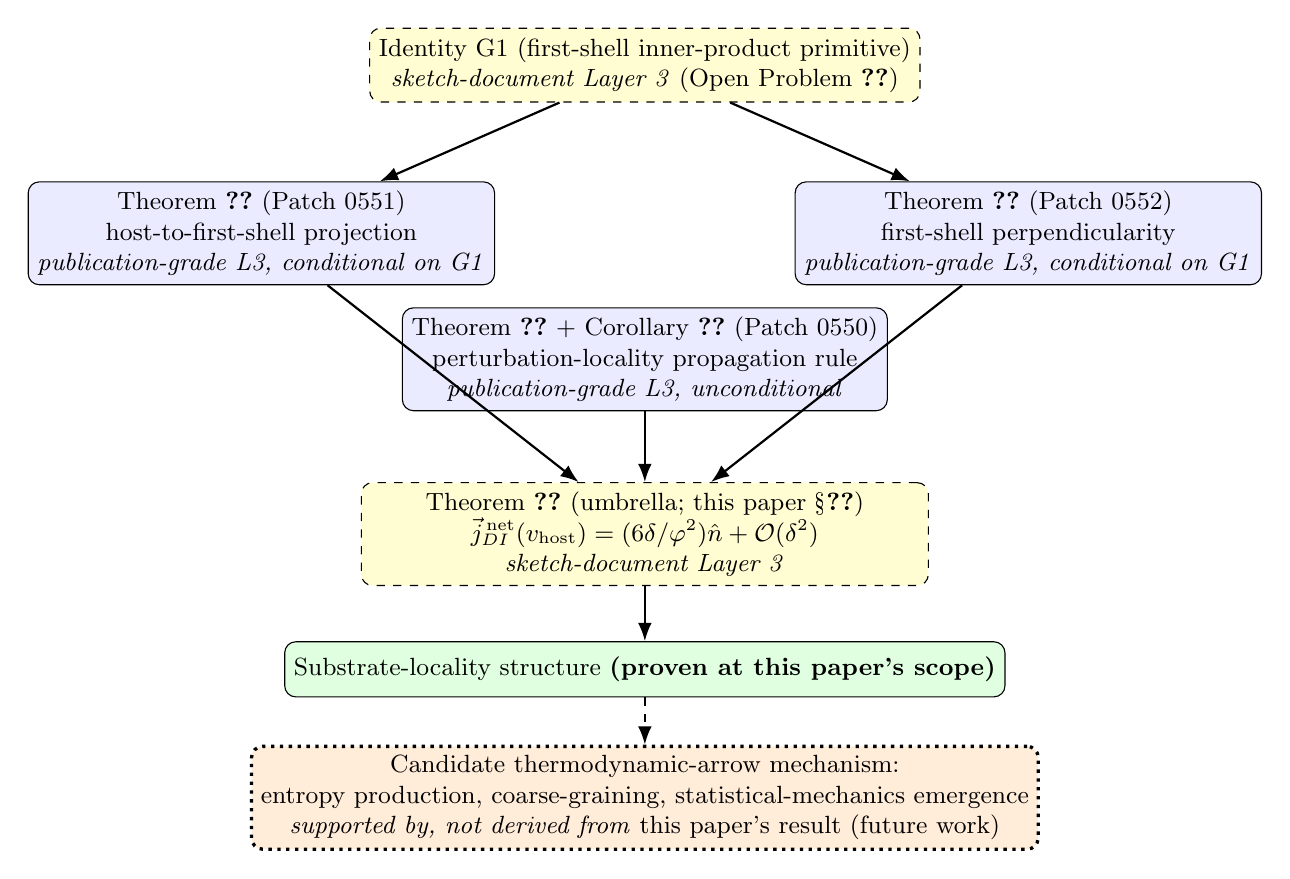
\begin{tikzpicture}[
  every node/.style={align=center, font=\small},
  pub/.style={rectangle, draw, fill=blue!8, minimum height=0.7cm, minimum width=5.6cm, rounded corners},
  sketch/.style={rectangle, draw, fill=yellow!18, minimum height=0.7cm, minimum width=5.6cm, rounded corners, dashed},
  umbrella/.style={rectangle, draw, fill=yellow!18, minimum height=1.0cm, minimum width=7.2cm, rounded corners, dashed},
  proven/.style={rectangle, draw, fill=green!12, minimum height=0.7cm, minimum width=7.2cm, rounded corners},
  cand/.style={rectangle, draw, fill=orange!15, minimum height=1.0cm, minimum width=8.8cm, rounded corners, dotted, very thick},
  arr/.style={-Latex, thick},
  arrcand/.style={-Latex, thick, dashed}
]
% Top: G1
\node[sketch] (g1) {Identity G1 (first-shell inner-product primitive) \\ \emph{sketch-document Layer 3} (Open Problem~\ref{op:g1-hardening})};
% Row 2: Theorems 5.1, 5.2 (left, right) and 6.1 (below)
\node[pub, below left=1.0cm and -1.6cm of g1] (t51) {Theorem~\ref{thm:host-first-shell-projection} (Patch 0551) \\ host-to-first-shell projection \\ \emph{publication-grade L3, conditional on G1}};
\node[pub, below right=1.0cm and -1.6cm of g1] (t52) {Theorem~\ref{thm:first-shell-perpendicularity} (Patch 0552) \\ first-shell perpendicularity \\ \emph{publication-grade L3, conditional on G1}};
\node[pub, below=2.6cm of g1] (t61) {Theorem~\ref{thm:perturbation-locality} + Corollary~\ref{cor:shell-locality} (Patch 0550) \\ perturbation-locality propagation rule \\ \emph{publication-grade L3, unconditional}};
% Row 3: Theorem 7.1 umbrella
\node[umbrella, below=0.9cm of t61] (t71) {Theorem~\ref{thm:substrate-locality} (umbrella; this paper \S\ref{sec:substrate-locality-theorem}) \\ $\jDInet(\vhost) = (6\delta/\phig^2)\hat{n} + \bigO{\delta^2}$ \\ \emph{sketch-document Layer 3}};
% Row 4: Substrate-locality structure (proven)
\node[proven, below=0.7cm of t71] (sl) {Substrate-locality structure \textbf{(proven at this paper's scope)}};
% Row 5: Candidate mechanism
\node[cand, below=0.6cm of sl] (cand) {Candidate thermodynamic-arrow mechanism: \\ entropy production, coarse-graining, statistical-mechanics emergence \\ \emph{supported by, not derived from} this paper's result (future work)};
% Arrows
\draw[arr] (g1) -- (t51);
\draw[arr] (g1) -- (t52);
\draw[arr] (t51) -- (t71);
\draw[arr] (t52) -- (t71);
\draw[arr] (t61) -- (t71);
\draw[arr] (t71) -- (sl);
\draw[arrcand] (sl) -- (cand);
\end{tikzpicture}
\caption{Dependency graph of the F.1 flagship paper's theorem stack. \emph{Solid arrows} indicate mathematical dependency (proven inference); the \emph{dashed arrow} at the bottom indicates supported-but-not-derived (the candidate mechanism narrative). Identity G1 supports Theorems~\ref{thm:host-first-shell-projection} and~\ref{thm:first-shell-perpendicularity}; together with the unconditional Theorem~\ref{thm:perturbation-locality}~+~Corollary~\ref{cor:shell-locality}, the trio is assembled into the umbrella Theorem~\ref{thm:substrate-locality} (sketch-document Layer 3) and the substrate-locality structure it proves. The further step from substrate-locality structure to thermodynamic-arrow emergence (entropy production, coarse-graining, statistical-mechanics) is the candidate mechanism narrative, \emph{supported by but not derived from} the present paper's result; it is registered as future work beyond the present paper's framework qualifiers. The figure complements Table~\ref{tab:layer-hierarchy} with the visual dependency structure.}
\label{fig:dependency-graph}
\end{figure}

Table~\ref{tab:layer-hierarchy} encodes the per-theorem rigor classification operationalised at \S\S\ref{sec:framework-primitives}--\ref{sec:substrate-locality-theorem}; Figure~\ref{fig:dependency-graph} renders the same information as a dependency graph. Three structural readings:

First, the publication-grade trio at Patches~0550--0552 anchors the paper's load-bearing geometric and perturbation-theory content. Closing exclusion class~E1 (Open Problem~\ref{op:g1-hardening}; G1 publication-grade hardening) would upgrade Theorems~\ref{thm:host-first-shell-projection} and~\ref{thm:first-shell-perpendicularity} (and consequently Lemma~\ref{lem:chord-length}) to unconditional publication-grade Layer~3. Theorem~\ref{thm:perturbation-locality} and Corollary~\ref{cor:shell-locality} are already at unconditional publication-grade Layer~3.

Second, the sketch-document umbrella Theorem~\ref{thm:substrate-locality} sits one Layer level below the trio. Its dependencies on G1 and on the trio mean that closing op:g1-hardening alone is insufficient to upgrade the umbrella; a separate publication-grade hardening of Theorem~\ref{thm:substrate-locality} (a candidate follow-up Patch beyond the paper's scope) would be needed.

Third, the framework-axiom Axioms MA.1 + MA.2 sit at a distinct Layer position --- not a derived statement at any Layer, but a framework-axiom input. Their derivation from CPP primitive axioms A1--A11 is at Layer~4 (Open Problem~\ref{op:layer4-mechanism-a}); this is the long-term programme target, not a paper-level closure item.

\subsection{Implications for the Layer 4 trajectory and the F.1 sub-question status}
\label{sec:layer4-implications}

The Layer-3 stack of Table~\ref{tab:layer-hierarchy} has three implications for the Layer-4 trajectory:

\paragraph{Implication 1: G1 hardening unlocks Theorem~7.1 conditionality.}
Closing Open Problem~\ref{op:g1-hardening} (G1 publication-grade hardening) would upgrade the trio to unconditional publication-grade Layer~3, removing the G1 dependency from the umbrella theorem's conditionality clause. Theorem~\ref{thm:substrate-locality} would then be at sketch-document Layer~3 \emph{conditional only on the trio} (which would itself be unconditional). A subsequent publication-grade hardening Patch of Theorem~\ref{thm:substrate-locality} would then upgrade the umbrella to unconditional publication-grade Layer~3 outright.

\paragraph{Implication 2: Layer~4 axiomatic derivation is independent of G1 hardening.}
The Layer~4 derivation of Mechanism~A (Open Problem~\ref{op:layer4-mechanism-a}; derivation of Axioms MA.1 + MA.2 from CPP primitive axioms A1--A11) is a separate trajectory from G1 publication-grade hardening (Open Problem~\ref{op:g1-hardening}). Closing one does not affect the other; the two Open Problems can be pursued in parallel or in either order without dependency conflict.

\paragraph{Implication 3: The F.1 sub-question is at "structurally-grounded sketch-document Layer~3 closure".}
The Patch~0549 framing of the F.1 sub-question's status --- ``\emph{structurally-grounded sketch-document Layer~3 closure under the Reading~C + 600-cell + Mechanism~A minimal-local-first-order framework, pending Layer~4 axiomatic derivation, $\bigO{\delta^2}$ extension, and publication-grade hardening of identity G1}'' --- is exactly the closure level achieved by Theorem~\ref{thm:substrate-locality} (\S\ref{sec:substrate-locality-theorem}) under the framework qualifiers of \S\ref{sec:statement-assembly}. The three pending items are: (i) Layer~4 axiomatic derivation (Open Problem~\ref{op:layer4-mechanism-a}); (ii) $\bigO{\delta^2}$ extension (Open Problem~\ref{op:delta-squared}); (iii) G1 publication-grade hardening (Open Problem~\ref{op:g1-hardening}). None is required for the substrate-locality umbrella to hold at sketch-document Layer~3 at the present paper's scope; all three are registered as open problems for the F.1 sub-question's broader closure to higher Layer or extended scope.

\paragraph{Anti-erasure discipline.}
Table~\ref{tab:layer-hierarchy} sustains the anti-erasure discipline that has guided the paper from \S\ref{sec:framework-primitives} forward: every per-theorem Layer label, every conditionality clause, every exclusion class reference, and every source-artifact reference is preserved in the unified table. The table is the place a reviewer can verify in one read that every result's rigor and dependency structure is explicit. The discipline is operational at the theorem-statement level (parenthetical Layer labels) and at the table level (Table~\ref{tab:layer-hierarchy}); both layers of representation are sustained without erasure.

% ============================================================
% §9 Open higher-order questions
%   Body to be added at Patch 0563.
%   Primary source: Patch 0549 §38.3 + the three .tex artifacts'
%   E-class lists.
%   Approximate target: 2-3 pages.
% ============================================================
\section{Open higher-order questions}
\label{sec:open-questions}

% [Body added at Patch 0564 per scoping doc §4.2 ninth step.
%  Multi-block substitution covering §9 inner placeholder + 5 Open Problem
%  environment placeholders. Each Open Problem parenthetical title and
%  label preserved unchanged from skeleton per Patch 0563 forward queue
%  instruction. Primary source: Patch 0549 §38.3 + the three hardened
%  theorems' five-class exclusion enumerations.]

This section presents the five open questions registered at the present paper's scope as Open Problems OPEN-FP-F1-1 through OPEN-FP-F1-5. The five questions span the conditionality structure of the umbrella theorem (G1 hardening, Theorem~7.1's unconditional status), the higher-order extension ($\bigO{\delta^2}$ corrections), the long-term axiomatic derivation (Layer~4), the chirality continuum's broader manifestation domain (sector-5 schema), and the present paper's Reading~C scope restriction (non-vertex-aligned variants). All five are referenced in earlier sections where their resolution would clarify or extend a claim; here we collect their statements in unified form for the reader and for future trajectory planning.

\begin{openproblem}[Extension to $\bigO{\delta^2}$; OPEN-FP-F1-1]
\label{op:delta-squared}
The substrate-locality umbrella theorem (Theorem~\ref{thm:substrate-locality}) closes the F.1 sub-question at first order in $\delta$. Higher-order corrections at $\bigO{\delta^2}$ and beyond are deferred. By Theorem~\ref{thm:perturbation-locality} (perturbation-theory propagation rule), the $\bigO{\delta^2}$ coefficient $\vec{J}_2(\vhost)$ depends only on edges in the 2-ball $E_2(\vhost)$ of the 600-cell edge graph --- the 12 host-to-first-shell edges + 30 first-shell-to-first-shell edges + 60 first-shell-to-second-shell edges + various second-shell-to-second-shell edges. The geometric structure of the 600-cell second shell (20 vertices forming a regular dodecahedron at distance $\sqrt{2 - 2 \cos(72^\circ)} = 1/\phig \cdot \sqrt{3 - \phig}$ from $\vhost$) is well-characterised, but the second-shell inner-product structure and edge-direction projection identities analogous to G1 + G2 + Theorem~\ref{thm:host-first-shell-projection} have not been worked out. Closure of OPEN-FP-F1-1 would (i) derive the second-shell inner-product and edge-projection identities; (ii) extend Theorem~\ref{thm:substrate-locality} to a closed-form expression for $\jDInet(\vhost)$ at $\bigO{\delta^2}$; (iii) examine whether second-shell content introduces tangent-direction components to $\jDInet(\vhost)$ (i.e., whether the parallel-to-$\hat{n}$ structure of Equation~\eqref{eq:substrate-locality} survives at second order). This is a substantive geometric and perturbation-theory project; methodologically analogous to the present paper but at higher order, with computational effort scaled by the second-shell edge count.
\end{openproblem}

\begin{openproblem}[Layer 4 axiomatic derivation of Mechanism A; OPEN-FP-F1-2]
\label{op:layer4-mechanism-a}
Mechanism~A is taken as framework axiom (Axioms MA.1 + MA.2 of \S\ref{sec:mechanism-a}) at the present paper's scope. The propagation-rate asymmetry $r(\hat{e}) = r_0(1 + \delta\,\hat{e}\cdot\hat{n})$ and the framework-local current construction at $\bigO{\delta^1}$ are independent commitments at Layer~3 framework input. Closure of OPEN-FP-F1-2 would derive Mechanism~A from the CPP primitive axioms A1--A11 alone. Specifically: derive the propagation-rate asymmetry from the CP + DI-bit + PCD-cycle primitives of A1 + A6$^{\prime}$ (CPs interconnected by DI-bits as elementary information units; PCD cycle as elementary discrete-time temporal process); derive the vertex-uniformity of the rate (its independence of the originating vertex $v$) from the substrate's discrete geometric structure A11 (600-cell substrate). The derivation is the long-term programme target. Its closure would unlock unconditional Layer~4 axiomatic status for Theorem~\ref{thm:substrate-locality} (and hence for the F.1 sub-question's closure), discharging the framework-axiom conditionality to the primitive-axiom level. The derivation is anticipated to be substantial --- spanning multiple Patches in a dedicated trajectory --- and is not pursued at the present paper's scope.
\end{openproblem}

\begin{openproblem}[Publication-grade hardening of identity G1; OPEN-FP-F1-3]
\label{op:g1-hardening}
Identity G1 (first-shell inner-product primitive; Lemma~\ref{lem:g1-imported}) is at sketch-document Layer~3 rigor in the present paper (imported from Patch~0541 \S3.1 with derivation from the 600-cell first-shell-edge dihedral angle $\cos(36^\circ) = \phig/2$ + unit-vertex normalisation). The publication-grade hardening of G1 --- with explicit hypothesis tracking, isolation of the dihedral-angle calculation as a standalone lemma, the icosahedral residual symmetry $H_3 = I_h$ as a separately-derived structural input, and a five-class exclusion enumeration --- is the shared exclusion class~E1 of Theorems~\ref{thm:host-first-shell-projection} and~\ref{thm:first-shell-perpendicularity} (Patches~0551 + 0552 hardened-theorem artifacts). Closure of OPEN-FP-F1-3 would proceed by a dedicated G1 hardening Patch producing a `hardened\_theorems/' artifact (e.g., \texttt{first\_shell\_inner\_product\_primitive.tex}) parallel in structure to the three existing hardened artifacts. Closure would upgrade Theorems~\ref{thm:host-first-shell-projection} and~\ref{thm:first-shell-perpendicularity} from \emph{publication-grade Layer~3 conditional on G1} to \emph{publication-grade Layer~3 unconditional}, and consequently upgrade Theorem~\ref{thm:substrate-locality}'s conditionality clause to depend only on the trio (which would itself be unconditional). The G1 hardening can be pursued independently of and prior to OPEN-FP-F1-1 (higher-order extension) and OPEN-FP-F1-2 (Layer~4 derivation); the three Open Problems are independent.
\end{openproblem}

\begin{openproblem}[Sector-5 schema instantiation; OPEN-FP-F1-4]
\label{op:sector5-schema}
The chirality continuum architecture (Capotauro~v2.0 + chirality continuum sketch document) anticipates that the substrate-direction primitive $\hat{n}$ manifests across multiple sectors of the CPP corpus. The present paper's manifestation~(iv) (thermodynamic causal arrow via substrate-locality of DI-bit currents) joins Capotauro~v2.0's spatial-sector manifestations~(i)--(iii) (parity violation, neutrino chirality structure, weak isospin assignment) as the second sector explicitly closed. Closure of OPEN-FP-F1-4 would identify manifestation~(v) of the substrate primitive --- the conjectured ``Sector~5'' --- and provide a sketch-document-level realisation analogous to the present paper's Theorem~\ref{thm:substrate-locality}. Candidate domains for Sector~5 (discussed at Patch~0549 \S38.3) include: thermal-equilibrium gauge fixing in finite-temperature field theory; symmetry-restoration dynamics at the electroweak crossover; cosmological-arrow alignment in the CPP-cosmology trajectory. None of these is committed; the question is open and substantive. Closure is contingent on identifying the structural manifestation, which is itself a research-direction-choosing question, not a derivation question.
\end{openproblem}

\begin{openproblem}[Non-vertex-aligned Reading C variants; OPEN-FP-F1-5]
\label{op:non-vertex-aligned-c}
The present paper uses \emph{vertex-aligned Reading~C} exclusively (Equation~\eqref{eq:reading-c-alignment}: $\hat{n} = \vhost / |\vhost| = \vhost$). Two other Reading~C variants exist within the 600-cell substrate: \emph{edge-aligned Reading~C} (with $\hat{n}$ along a 600-cell short-edge direction, giving residual $D_3$ symmetry at the edge midpoint); \emph{face-aligned Reading~C} (with $\hat{n}$ perpendicular to a triangular face, giving residual $D_2$ symmetry at the face centroid). Capotauro~v2.0 §2.3 + Patch~0419 Finding~C-W37 frame these as three sub-cases of a single Reading~C primitive class, with vertex-aligned being the most symmetric. The first-shell geometric primitives G1 + G2 are specific to vertex-aligned Reading~C: the dihedral angle $36^\circ$ + icosahedral residual symmetry $H_3 = I_h$ at the host vertex are vertex-specific structural facts. For edge-aligned or face-aligned Reading~C, different residual symmetries ($D_3$ or $D_2$) and different first-shell geometric structures apply. Closure of OPEN-FP-F1-5 would extend (or reformulate) Theorems~\ref{thm:host-first-shell-projection}, \ref{thm:first-shell-perpendicularity}, and \ref{thm:substrate-locality} under the edge-aligned and face-aligned Reading~C variants. Whether the substrate-locality structure survives, fails, or takes a modified form (e.g., with a different structural constant replacing $6/\phig^2$, or with non-parallel-to-$\hat{n}$ components) is an open question. Methodologically, the closure proceeds by replaying §3--§7 with the alternative residual-symmetry structures; the computational effort is moderate but the conceptual novelty (identifying which 600-cell geometric identities are reading-C-specific vs reading-C-independent) is substantive.
\end{openproblem}

The five Open Problems are independent at first order: closing any one does not constrain or unlock the others, with one exception --- OPEN-FP-F1-3 (G1 hardening) interacts with the conditionality clauses of Theorems~\ref{thm:host-first-shell-projection}, \ref{thm:first-shell-perpendicularity}, and (via the trio) Theorem~\ref{thm:substrate-locality}. The other four are mutually orthogonal. The forward trajectory of the F.1 programme prioritises OPEN-FP-F1-3 (the most immediately tractable; closes the load-bearing E1 exclusion of the §5 trio members) and OPEN-FP-F1-1 (the natural extension of the present paper's central result); OPEN-FP-F1-2 is the long-term programme target; OPEN-FP-F1-4 and OPEN-FP-F1-5 are research-direction-choosing questions registered for future Patches in the broader chirality continuum and Reading~C-variant trajectories.

% ============================================================
% §10 Conclusion
%   Body to be added at Patch 0564.
%   Ties Layer 3 closure to CPP chirality-from-polytope-geometry
%   long-term programme target (Patch 0528 §14.17 + Patch 0539 §15.5).
%   Approximate target: 1-2 pages.
% ============================================================
\section{Conclusion}
\label{sec:conclusion}

% [Body added at Patch 0565 per scoping doc §4.2 tenth (final body) step.
%  Not an integration Patch. Synthesises F.1 sub-question closure and ties
%  to CPP chirality-from-polytope-geometry long-term programme target
%  (Patch 0528 §14.17 + Patch 0539 §15.5 as referenced in skeleton outer
%  comment header). The §10 placeholder is sparse — no anticipated
%  sub-structure provided. Structure designed: substantive synthesis,
%  position in chirality continuum, long-term programme connection,
%  forward trajectory. Target 1-2 pages.]

The present paper establishes structurally-grounded sketch-document Layer~3 closure of the F.1 sub-question under the Reading~C + 600-cell + Mechanism~A minimal-local-first-order framework. The substantive closure result, Theorem~\ref{thm:substrate-locality} (Equation~\eqref{eq:substrate-locality}), reduces the net DI-bit current at the host vertex $\vhost$ at first order in $\delta$ to the closed-form expression
\[
\jDInet(\vhost) = \frac{6 \delta}{\phig^2} \, \hat{n} + \bigO{\delta^2},
\]
exhibiting substrate-locality (first-shell-only dependence) and parallel-to-$\hat{n}$ structure at $\bigO{\delta^1}$. The structural constant $6/\phig^2 \approx 2.2918$ joins the temporal sector to the chirality continuum's spatial sector (Capotauro v2.0~\S3), where parallel structural constants govern the substrate primitive's manifestations~(i)--(iii) (parity violation, neutrino chirality, weak isospin assignment). The closure is at the \emph{substrate-locality level} --- the closed-form structure of the DI-bit current at first order in $\delta$. The further step from substrate-locality structure to thermodynamic-arrow emergence in the conventional physics sense (entropy production, irreversible coarse-graining, statistical-mechanics arrow) is the candidate mechanism narrative supported by, but not derived from, the present paper's result; the emergence layer is registered as future work beyond the present paper's framework qualifiers.

The paper's substantive contribution decomposes into two parts. \emph{First}, the publication-grade hardening of the three building-block theorems (\S\ref{sec:first-shell-identities} + \S\ref{sec:perturbation-locality}; Patches~0550--0552 hardened-theorem trio at \texttt{hardened\_theorems/}): Theorems~\ref{thm:host-first-shell-projection}, \ref{thm:first-shell-perpendicularity}, \ref{thm:perturbation-locality}, and Corollary~\ref{cor:shell-locality} are at publication-grade Layer~3 rigor with explicit hypothesis tracking and five-class exclusion enumerations. \emph{Second}, the assembly of the trio into the substrate-locality umbrella theorem (\S\ref{sec:substrate-locality-theorem}; Theorem~\ref{thm:substrate-locality}) at sketch-document Layer~3, with the closed-form result depending on only first-shell content at first order. The two parts together --- publication-grade trio plus sketch-document umbrella --- form the Layer~3 stack of \S\ref{sec:layer3-stack} (Table~\ref{tab:layer-hierarchy}).

The closure is conditional on three pending items registered as Open Problems (\S\ref{sec:open-questions}): publication-grade hardening of identity G1 (Open Problem~\ref{op:g1-hardening}; the shared exclusion class~E1 of the §5 hardened theorems); extension to $\bigO{\delta^2}$ and beyond (Open Problem~\ref{op:delta-squared}; the natural higher-order extension of Theorem~\ref{thm:substrate-locality}); Layer~4 axiomatic derivation of Mechanism~A from CPP primitive axioms A1--A11 (Open Problem~\ref{op:layer4-mechanism-a}; the long-term programme target). None of these is required for the substrate-locality umbrella to hold at sketch-document Layer~3 at the present paper's scope; all three are registered as open problems for the F.1 sub-question's broader closure to higher Layer or extended scope. Two additional Open Problems --- Sector-5 schema instantiation (Open Problem~\ref{op:sector5-schema}) and non-vertex-aligned Reading~C variants (Open Problem~\ref{op:non-vertex-aligned-c}) --- are research-direction-choosing questions for the broader chirality continuum and Reading~C-variant trajectories.

\paragraph{Position in the CPP chirality-from-polytope-geometry long-term programme.}
The present paper's result is the second sector closure of the broader CPP chirality-from-polytope-geometry programme target (Patch~0528 \S14.17; Patch~0539 \S15.5). The programme target, in summary, is: \emph{the chirality structure of physical law arises from the discrete geometric primitives of the 600-cell substrate at Reading~C, with the substrate primitive $\hat{n}$ as the unifying direction across multiple sectors of physical manifestation.} Capotauro v2.0's spatial-sector closure (manifestations (i)--(iii) at \S3) and the present paper's temporal-sector closure (manifestation (iv)) provide two of the anticipated sectoral closures; Open Problem~\ref{op:sector5-schema} registers the next-sector identification as the natural forward trajectory.

The structural constant $-1/(2\phig)$ shared between Capotauro~v2.0's spatial-sector substrate-locality theorem (\S3 of that paper) and the present paper's Theorem~\ref{thm:host-first-shell-projection} is not a numerical coincidence; it is the imprint of the same first-shell geometric content (Identity~G1 + Identity~G2 + the 600-cell host-vertex stabiliser $H_3 = I_h$) operating across both sectors. The chirality continuum's two-sector umbrella structure --- spatial $+$ temporal --- is anchored at the polytope-geometric level by this shared structural content. The closed-form coefficient $6/\phig^2$ of Equation~\eqref{eq:substrate-locality}, derived from $-1/(2\phig)$ via the icosahedral-sum identity at \S\ref{sec:proof-from-5-6}, is the temporal-sector specialisation of that shared content.

\paragraph{Forward trajectory.}
The F.1 sub-question's closure at the present paper's Layer~3 scope opens four trajectories for follow-up work, in approximate order of immediate tractability: (i) G1 publication-grade hardening (Open Problem~\ref{op:g1-hardening}); (ii) substrate-locality umbrella publication-grade hardening (a candidate follow-up Patch beyond the present paper's scope, not registered as a formal Open Problem); (iii) $\bigO{\delta^2}$ extension (Open Problem~\ref{op:delta-squared}); (iv) Layer~4 axiomatic derivation of Mechanism~A (Open Problem~\ref{op:layer4-mechanism-a}). Trajectories (i)--(iii) operate within the present paper's framework qualifiers; trajectory (iv) discharges Mechanism~A to the CPP primitive axiom level. Beyond these, the F.2 and F.3 sub-questions of the broader F-series provide additional substrate-direction-primitive sub-questions whose closure is anticipated to follow analogous Layer-3 closure patterns.

The chirality continuum's broader sectoral programme (Open Problem~\ref{op:sector5-schema} and beyond) and the Reading~C-variant programme (Open Problem~\ref{op:non-vertex-aligned-c}) operate at scope levels above the present paper's framework qualifiers; their closure trajectories are research-direction-choosing rather than derivation, and are registered for future programme-direction Patches in the broader CPP corpus.

The substantive result of the present paper is the temporal-sector substrate-locality theorem; the broader contribution is the demonstration that the 600-cell polytope geometry, at vertex-aligned Reading~C with Mechanism~A as framework axiom, produces a closed-form physical-content claim at $\bigO{\delta^1}$ that joins Capotauro~v2.0's spatial-sector closure as the second pillar of the chirality continuum's polytope-geometric foundation. The publication-grade rigor at the trio level and the sketch-document Layer~3 closure at the umbrella level together represent the level of substantive contribution targeted by the F.1 trajectory at Patch~0549; the broader programme target (chirality from polytope geometry, with $\hat{n}$ as the unifying direction across multiple sectors) is one sector closer to its long-term completion.

% ============================================================
% Bibliography
%   Body to be added at Patch 0565.
%   Imports from bibliography/cpp_references.bib + adds F.1-specific
%   entries.
% ============================================================
\bibliographystyle{plain}
% \bibliography{../../bibliography/cpp_references}  % uncomment at Patch 0565
\begin{thebibliography}{99}

% [Bibliography entries populated at Patch 0566.
%  Note on style: the paper body uses inline parenthetical references
%  (e.g., "Capotauro v2.0", "Patch 0541 §3.1") rather than \cite{} commands.
%  The \bibitem{} entries below serve as a formal references list for the
%  corpus material mentioned inline. Switch to \cite{} integration is a
%  candidate Patch 0567 (final polish) decision if the editor / reviewer
%  prefers conventional citation style. Patch 0567 candidate also includes
%  the option of uncommenting \bibliography{../../bibliography/cpp_references}
%  to use the corpus BibTeX file directly; for the present Patch we use
%  explicit \bibitem{} entries to preserve the body content unchanged.]

\bibitem{chirality-continuum-v2}
T.~L.~Abshier,
``Chirality Continuum from Substrate to Observable EFT: Joint Layer 4 Closure of OPEN-FP-SF-2-CHIR (Electroweak V--A Coupling) and SM-2 v2.0+ (Quark Chiral-Polarity-Bias) from $|M| = \chi/6$,''
Hyperphysics Institute, v1.0 SHIPPED 20 May 2026, Session 137 Patch~0509,
DOI: 10.17605/OSF.IO/JXE8D, 2026.

\bibitem{patch-0419-reading-c}
T.~L.~Abshier (with Claude Opus),
``Finding C-W37: Vertex-aligned, edge-aligned, and face-aligned Reading~C variants in the 600-cell substrate,''
CPP corpus record, Patch~0419, Hyperphysics Institute, 2026.

\bibitem{patch-0528-programme-target}
T.~L.~Abshier (with Claude Opus),
``CPP Chirality-from-Polytope-Geometry Long-Term Programme Target,''
CPP corpus record, Patch~0528 \S14.17, Hyperphysics Institute, 2026.

\bibitem{patch-0539-programme-target}
T.~L.~Abshier (with Claude Opus),
``Chirality-from-polytope-geometry programme structure update,''
CPP corpus record, Patch~0539 \S15.5, Hyperphysics Institute, 2026.

\bibitem{patch-0541-primitives}
T.~L.~Abshier (with Claude Opus),
``Foundational geometric primitives for the F.1 sub-question trajectory: 600-cell first-shell identity~G1 (first-shell inner-product primitive $v_i \cdot v_{\text{host}} = \phi/2$) at sketch-document Layer~3 rigor,''
CPP corpus record, Patch~0541 \S3.1, Hyperphysics Institute, 2026.

\bibitem{patch-0544-mechanism-a}
T.~L.~Abshier (with Claude Opus),
``Mechanism~A formalisation: propagation-rate asymmetry $r(\hat{e}) = r_0(1 + \delta\,\hat{e}\cdot\hat{n})$ and the framework-local current construction at sketch-document Layer~3 rigor,''
CPP corpus record, Patch~0544 \S3, Hyperphysics Institute, 2026.

\bibitem{patch-0549-status-framing}
T.~L.~Abshier (with Claude Opus),
``F.1 sub-question status framing: structurally-grounded sketch-document Layer~3 closure under the Reading~C + 600-cell + Mechanism~A minimal-local-first-order framework,''
CPP corpus record, Patch~0549 \S38.3, Hyperphysics Institute, 2026.

\bibitem{patch-0550-perturbation-locality}
T.~L.~Abshier (with Claude Opus),
``Perturbation-theory propagation rule for the framework-local DI-bit current in the 600-cell edge graph: $\mathcal{O}(\delta^n)$ coefficient confined to graph-distance-$n$ edges, hardened to publication-grade Layer~3,''
CPP corpus record, Patch~0550, Hyperphysics Institute, 2026.
Source artifact: \texttt{flagship\_papers/dynamical\_substrate\_law/hardened\_theorems/perturbation\_locality\_propagation.tex}.

\bibitem{patch-0551-first-shell-perpendicularity}
T.~L.~Abshier (with Claude Opus),
``First-shell-to-first-shell perpendicularity in the 600-cell at vertex-aligned Reading~C: $\hat{e}_{ij} \cdot \hat{n} = 0$, hardened to publication-grade Layer~3 conditional on G1,''
CPP corpus record, Patch~0551, Hyperphysics Institute, 2026.
Source artifact: \texttt{flagship\_papers/dynamical\_substrate\_law/hardened\_theorems/first\_shell\_perpendicularity.tex}.

\bibitem{patch-0552-host-first-shell-projection}
T.~L.~Abshier (with Claude Opus),
``Host-to-first-shell uniform projection in the 600-cell at vertex-aligned Reading~C: $\hat{u}_i \cdot \hat{n} = -1/(2\phi)$ exactly and uniformly across all 12 first-shell neighbours, hardened to publication-grade Layer~3 conditional on G1,''
CPP corpus record, Patch~0552, Hyperphysics Institute, 2026.
Source artifact: \texttt{flagship\_papers/dynamical\_substrate\_law/hardened\_theorems/host\_to\_first\_shell\_projection.tex}.

\bibitem{tatwd-book}
T.~L.~Abshier (with M.~Abshier),
``Tetrahedrons All the Way Down: Conscious Point Physics and the 600-Cell Substrate of Physical Reality,''
Hyperphysics Institute (book project), in preparation, 2026.
Chapter~3 provides the full statement of CPP primitive axioms A1--A11; cf.\ \texttt{templates/operating\_system.md} for the registry.

\bibitem{coxeter-regular-polytopes}
H.~S.~M.~Coxeter,
``Regular Polytopes,''
Dover Publications, New York, 3rd edition, 1973.
Standard reference for the 600-cell regular 4-polytope, $H_4$ symmetry group, and the icosahedral residual symmetry $H_3 = I_h$.

\bibitem{cpp-operating-system}
T.~L.~Abshier (with Claude Opus),
``CPP Theory Operating System: axiom registry, paper-completion checklist, and Layer-distinction discipline,''
\texttt{templates/operating\_system.md}, Hyperphysics Institute, 2026.
The authoritative source for CPP primitive axioms A1--A11 (recap in \S\ref{sec:cpp-axioms-recap}) and the Layer-distinction discipline operationalised throughout the paper.

\end{thebibliography}

\end{document}
